
\documentclass[conf]{new-aiaa}
\usepackage{graphicx}
\usepackage{amsmath}
\usepackage{authblk}
\usepackage{textcomp}
\usepackage{bm}
\usepackage[version=4]{mhchem}
\usepackage{siunitx}
\usepackage{longtable,tabularx}
\setlength\LTleft{0pt}
\usepackage{minted}
\usepackage{float}
\usepackage{caption}
\newminted{python}{%
    % options to customize output of pythoncode
    linenos,
    breaklines,
    fontsize=\footnotesize,
    frame=lines,
    tabsize=4
}
\title{Attitude Dynamics and Control of a Nano-Satellite Orbiting Mars}

\author{Landry Matthews\footnote{Graduate Student, Aerospace Engineering Sciences, University of Colorado Boulder.}}
\affil{University of Colorado Boulder, Boulder, CO, 80309}

\begin{document}

\maketitle

\begin{abstract}
This document outlines the work completed for Tasks 1 through 11 of the ASEN 5010 Capstone Project - Attitude Dynamics and Control of a nano-Satellite Orbiting Mars. These tasks focus on simulating and analyzing the orbit and attitude dynamics of a nano-satellite in low Mars orbit. Results are derived using Python-based simulation frameworks and validated through analytical and numerical approaches, as well as through Coursera.
\end{abstract}

\section{Nomenclature}

{\renewcommand\arraystretch{1.0}
\noindent\begin{longtable*}{@{}l @{\quad=\quad} l@{}}
$(\Omega,i,\theta)$  & (3-1-3) Euler angles \\
$[BN]$ & direction cosine matrix from $\mathcal{N}$ frame to $\mathcal{B}$ frame \\
$[C]^T$ & transpose of the matrix $[C]$ \\ 
$[I_{3x3}]$ & a 3x3 identity matrix \\
$[\tilde{\bm\omega}]$ & skew-symmetric matrix of the vector $\bm\omega$ \\
${}^B[I]$  & inertia tensor $[I]$ expressed in $\mathcal{B}$ frame components \\
${}^B\bm u$ & control torque vector expressed in $\mathcal{B}$ frame components \\
${}^B\bm\omega_{R/N}$ & angular velocity of the $\mathcal{R}$ frame with respect to the $\mathcal{N}$ frame, expressed in $\mathcal{B}$ frame components \\
${}^N\bm r$ & vector $\bm r$ expressed in $\mathcal{N}$ frame components \\
$|\bm r|$ & magnitude/norm of the vector $\bm r$ \\ 
$\beta$ & quaternion \\
$\bm {}^BH$   & angular momentum vector $\bm H$ expressed in $\mathcal{B}$ frame components \\
$\bm r^T$ & transpose of the vector $\bm r$ \\ 
$\bm X$ & state vector \\
$\bm\sigma^S$ & the shadow MRP set of $\bm\sigma$ \\
$\bm\sigma_{B/N}$ & modified Rodrigues parameters from $\mathcal{N}$ frame to $\mathcal{B}$ frame \\
$\sigma^2$ & the same as $\bm\sigma^T\bm\sigma$\\
$\sigma_i$ & the $i$th component of the MRP set $\bm\sigma$ \\
$\dot\theta$ & derivative of $\theta$ \\
$\hat{\bm n}_1$ & unit vector of a frame (e.g. $\mathcal{N}$ frame) \\
$\mathcal{B}$ & spacecraft body frame - also seen as $B$ \\
$\mathcal{H}$ & orbital Hill frame - also seen as $H$ \\
$\mathcal{N}$ & mars centered inertial frame - also seen as $N$ \\
$\mathcal{O} : \{{\hat{\bm{i}}_r, \hat{\bm{i}}_{\theta}, \hat{\bm{i}}_h}\}$ & coordinate frame $\mathcal{O}$ (also seen as $O$) defined with three unit vector directions $\{{\hat{\bm{i}}_r, \hat{\bm{i}}_{\theta}, \hat{\bm{i}}_h}\}$ \\
$\mathcal{R}$ & generic spacecraft reference frame - also seen as $R$ \\
$\mathcal{R}_c$ & GMO-pointing communication reference frame - also seen as $R_c$ \\
$\mathcal{R}_n$ & nadir-pointing reference frame - also seen as $R_n$ \\
$\mathcal{R}_s$ & sun-pointing reference frame - also seen as $R_s$ \\
$\mu$ & gravitational constant \\
$\xi$ & damping ratio \\
$K$ & scalar attitude feedback gain \\
$P$ & scalar angular velocity feedback gain \\
$t$ & time \\
$T$ & rotational kinetic energy \\
DCM  & direction cosine matrix \\
GMO & geosynchronous Mars orbit satellite \\
J & Joules \\
kg & kilograms \\
LMO & low Mars orbit satellite \\
m & meters \\
MRPs & modified Rodrigues parameters \\
PD & proportional-derivative control \\
RK4 & Runge-Kutta 4th order integrator \\
s & seconds \\
\end{longtable*}}


\section{Introduction}
This project involves the design and implementation of an attitude control system for a small nano-satellite in a circular low Mars orbit (LMO). The satellite performs three key mission functions: gathering science data by pointing a sensor nadir towards Mars, recharging via solar panels by pointing its solar array towards the Sun, and transmitting data to a geosynchronous Mars orbit (GMO) mother satellite by aligning its communication platform.

We assume the Mars-inertial frame $\mathcal{N}$ and Hill frame $\mathcal{H} = \{\hat{\bm{i}}_r, \hat{\bm{i}}_{\theta}, \hat{\bm{i}}_h\}$ base vectors are as shown in the following figure.\begin{figure}[H]
    \centering
    \captionsetup{width=.7\linewidth}
    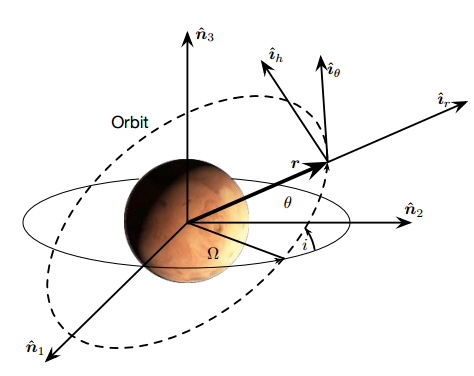
\includegraphics[width=.75\linewidth]{fig1.png}
    \caption{Illustration of the Inertial frame $\mathcal{N}$ and Hill frame $\mathcal{H}$ base vectors, with the vector $\bm r$ showing the position of the craft in orbit}
    \label{fig:enter-label}
\end{figure}
The attitude of the satellite is controlled using a thruster-based system that orients the spacecraft body frame $\mathcal{B}$ to align with a reference frame $\mathcal{R}$, which changes depending on the current operational mode (science, charging, or communication). These reference frames are computed on the basis of the known orbital parameters of the spacecraft and mother satellite, as well as the Sun's position relative to Mars.

The primary objective is to implement a feedback control law that drives the spacecraft's attitude and angular velocity---described by the modified Rodrigues parameters (MRPs) $\bm{\sigma}_{\mathcal{B}/\mathcal{N}}$ and angular velocity $\bm{\omega}_{\mathcal{B}/\mathcal{N}}$---to track their corresponding reference values $\bm{\sigma}_{\mathcal{R}/\mathcal{N}}$ and $\bm{\omega}_{\mathcal{R}/\mathcal{N}}$. This control task includes computing the appropriate torque input $\bm{u}$ and switching between control modes based on the orbital position of the spacecraft.

We are given the initial attitude MRP set and angular velocity conditions:
\[
\bm{\sigma}_{B/N} =
\begin{bmatrix}
\phantom{-}0.3 \\ -0.4 \\ \phantom{-}0.5
\end{bmatrix}, \quad
{}^B\bm{\omega}_{B/N} =
\begin{bmatrix}
\phantom{-}1.00 \\ \phantom{-}1.75 \\ -2.20
\end{bmatrix} \text{deg/s}
\]
Additionally, our spacecraft's inertia tensor is also provided:
\[
{}^B[I] = {}^B\begin{bmatrix}
10 & 0 & 0 \\
0 & 5 & 0 \\
0 & 0 & 7.5
\end{bmatrix} \text{kg m\textsuperscript{2}}
\]

We are required to follow certain protocol for when to align our spacecraft $\mathcal{B}$ frame with our 3 reference $\mathcal{R}$ frames. Depicted below is a figure illustrating our spacecraft body frame, showing its 3 principal axes aligning with the instrument sensors, solar panel normal, and antenna:
\begin{figure}[H]
    \centering
    \captionsetup{width=.7\linewidth}
    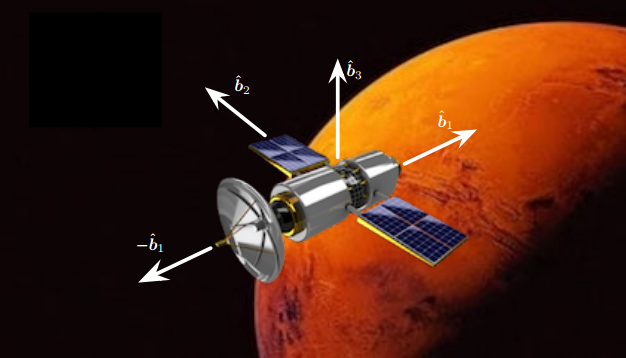
\includegraphics[width=.75\linewidth]{fig2.png}
    \caption{Illustration of the spacecraft's body frame $\mathcal{B}$ base vectors, showing the alignment of our subsystems of interest with our principal axes.}
    \label{fig:enter-label}
\end{figure}
During the mission, the spacecraft must follow a control protocol to stabilize its rotation and align its components along the desired reference axes. Specifically, the spacecraft will aim its antenna (along \( -\hat{\bm{b}}_1 \)) toward the GMO mother satellite when doing comm., its sensor (along \( \hat{\bm{b}}_1 \)) towards Mars (in the nadir or \( -\hat{\bm{r}} \) direction) when sampling science data, or its solar panels (along \( \hat{\bm{b}}_3 \)) toward the sun when charging. Given the telescope's high power consumption, the solar panels should always be pointed toward the sun when the spacecraft is on the sunlit hemisphere of Mars (i.e., when the \( \hat{\bm{n}}_2 \) coordinate is positive). Thus, the \( \hat{\bm{b}}_3 \) axis will be aligned with \( \hat{\bm{n}}_2 \) when the spacecraft is directed at the Sun. To complete the reference frame, the axis \( \hat{\bm{r}}_1 \) will point in the \( -\hat{\bm{n}}_1 \) direction.

When on the dark side of Mars (i.e., where the \( \hat{\bm{n}}_2 \) coordinate is negative), the spacecraft must switch to either communication or science mode. In science mode, the platform’s axis \( \hat{\bm{b}}_1 \) should point at Mars’ center, corresponding to the nadir direction. Additionally, the axis \( \hat{\bm{r}}_2 \) will align with the orbital track axis \( \hat{\bm{i}}_{\theta} \). In communication mode, the satellite needs to maintain a position where the angular separation between the LMO and GMO satellites is less than 35 degrees. If this angle is exceeded, we switch back to science mode. In this GMO facing mode, the communication axis \( -\hat{\bm{b}}_1 \) will be directed toward the GMO mother satellite. These mission pointing scenarios are summarized below in Table 1.

\begin{table}[h]
\centering
\caption{Spacecraft Pointing Scenario Summary}
\begin{tabular}{|c|c|}
\hline
\label{table1}
\textbf{Orbital Situation} & \textbf{Pointing Goals} \\ \hline
SC on sunlit side & Point \( \hat{\bm{b}}_3 \) at the Sun for Solar\\ \hline
SC on dark side \& GMO in sight & Point \( -\hat{\bm{b}}_1 \) at the GMO for comm. \\ \hline
SC on dark side \& GMO not in sight & Point \( \hat{\bm{b}}_1 \) nadir for sensors\\ \hline
\end{tabular}
\end{table}

The initial orbit frame angles of both the LMO and GMO satellites are listed in Table 2. The corresponding initial orbital positions are illustrated in Figure 3.

\begin{table}[h]
\centering
\caption{Initial Orbit Frame Orientation Angles}
\begin{tabular}{|c|c|c|c|}
\hline
\textbf{Spacecraft} & \( \Omega \) & \( i \) & \( \theta(t_0) \) \\ \hline
LMO & 0.349066 rad & 0.523599 rad & 1.0472 rad \\ \hline
GMO & 0 rad & 0 rad & 4.36332 rad \\ \hline
\end{tabular}
\end{table}
\begin{figure}[H]
    \centering
    \captionsetup{width=.7\linewidth}
    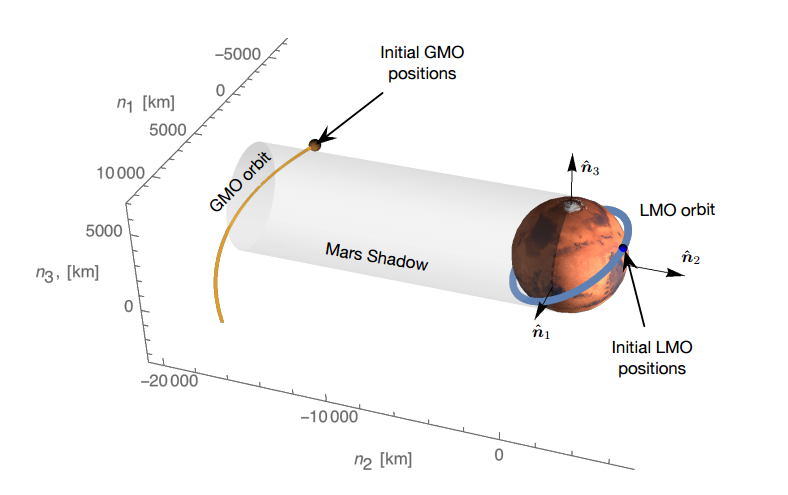
\includegraphics[width=.75\linewidth]{fig3.PNG}
    \caption{Illustration of the initial orbital positions of the LMO and GMO crafts, with the Mars centered inertial frame visible and with its $\hat{\bm n}_2$ axis pointing toward the Sun.}
    \label{fig:enter-label}
\end{figure}
Here we can see a visualization of the entire mission overview, showing that our LMO craft will start on the sunlit side of Mars before orbiting into the shadow. For simplicity, it is assumed that the sun is always positioned in the \( \hat{\bm{n}}_2 \) direction, as depicted in Figure 3.

We are also given a few more orbit characteristics:
The nano-satellite orbit has an altitude $h=400$ km, which when added to Mars' radius of $3396.19$ gives the LMO orbital radius of $r_{LMO} = 3796.19$ km. We are always given the GMO orbital radius of $r_{GMO} = 20424.2$ km, which is calculated via the fact that it is geosynchronous and thus must have the same 1 day and 37 minute orbital period as Mars' rotational period. 
To calculate the orbital rates, we are given Mars' gravity constant as $\mu = 42828.3$ km\textsuperscript{3}/s\textsuperscript{2}. 
The orbital rate of the LMO craft is then calculated through the equation $\dot{\theta}_{LMO} = \sqrt{u/r_{LMO}^3} = 0.000884797$ rad/s and the GMO craft via the same math giving $\dot{\theta}_{GMO} = \sqrt{u/r_{GMO}^3} = 0.0000709003$ rad/s. Since we are told they are in circular orbit, we know that $\dot{\theta}$ is constant for both crafts.

In this project, we employ a simple proportional-derivative (PD) attitude control law:

\[
{}^B\bm{u} = -K\bm{\sigma}_{B/R} - P{}^B\bm{\omega}_{B/R}
\]

This control law is used to drive the body frame \(\mathcal{B}\) towards its reference frame \(\mathcal{R}\). Note that both feedback gains \( P \) and \( K \) are scalars.

Throughout this project, practical experience is gained in reference frame generation, spacecraft attitude representation using MRPs, and the development of feedback controllers. The work involves both analytical derivations and implementation in simulation software, culminating in a full mission scenario demonstrating autonomous control switching.

It should be noted here that for all tasks, MRP calculations and results will always switch to the shadow set to avoid singularities when the shadow set condition $|\sigma| > 1$ is met. To switch we employ the shadow set equation
\[
\sigma^S_i = \frac{-\beta_i}{1-\beta_0} = \frac{-\sigma_i}{\sigma^2}, \qquad i=1,2,3 \tag{\cite{schaub},~eq. 3.147}
\]
I have written a helper function in Python \texttt{checkShadowSet(sigma)} which takes in the current MRP attitude set and returns the shadow set, if the condition is met. This function is called throughout all tasks where switching to shadow set is applicable. 

Each of the following tasks contributes to a component of this overall attitude control simulation.






\section{Task 1: Orbit Simulation}
For this task, we assume the general orbit frame \(\mathcal{N}\) is Mars-centered inertial. We also have the general orbit frame $\mathcal{O} : \{{\hat{\bm{i}}_r, \hat{\bm{i}}_{\theta}, \hat{\bm{i}}_h}\}$.

Next we had to write a function whose inputs are the radius \( r \) and the (3-1-3) Euler angles \( (\Omega, i, \theta) \), and whose outputs are the inertial position vector \( {}^N\mathbf{r} \) and velocity \( {}^N\dot{\mathbf{r}} \) of the associated circular orbit.

To do this, we start by writing two functions, \texttt{theta\_lmo(t)} and \texttt{theta\_gmo(t)}. They both work by simply computing and returning $\theta(t_0) + t \dot{\theta}$, which gives the updated value of $\theta$ for time $t$. Note that the $\theta$ values here are respective to LMO or GMO (depending on which function is called). 

From here, we can now obtain all 3 Euler angles for both our orbits at any time $t$. We can then write a helper function \texttt{Euler313toDCM(t1, t2, t3)}. Note for this function that $t1=\Omega,\ t2=i,\ $ and $t3 = \theta(t)$. This function converts 313 Euler angles to their corresponding directional cosine matrix (DCM). It uses the following DCM matrix written in terms of 313 Euler angles to do so (from Schaub and Junkins \cite{schaub} Appendix B):

\begin{gather}
 \label{euler}
    \begin{bmatrix}- \sin{\left(\Omega \right)} \sin{\left(\theta{\left(t \right)} \right)} \cos{\left(i \right)} + \cos{\left(\Omega \right)} \cos{\left(\theta{\left(t \right)} \right)} & \sin{\left(\Omega \right)} \cos{\left(\theta{\left(t \right)} \right)} + \sin{\left(\theta{\left(t \right)} \right)} \cos{\left(\Omega \right)} \cos{\left(i \right)} & \sin{\left(i \right)} \sin{\left(\theta{\left(t \right)} \right)}\\- \sin{\left(\Omega \right)} \cos{\left(i \right)} \cos{\left(\theta{\left(t \right)} \right)} - \sin{\left(\theta{\left(t \right)} \right)} \cos{\left(\Omega \right)} & - \sin{\left(\Omega \right)} \sin{\left(\theta{\left(t \right)} \right)} + \cos{\left(\Omega \right)} \cos{\left(i \right)} \cos{\left(\theta{\left(t \right)} \right)} & \sin{\left(i \right)} \cos{\left(\theta{\left(t \right)} \right)}\\\sin{\left(\Omega \right)} \sin{\left(i \right)} & - \sin{\left(i \right)} \cos{\left(\Omega \right)} & \cos{\left(i \right)}
    \end{bmatrix}
\end{gather}

Now that we have a function to convert from Euler angles to DCMs, and a function to get our $\theta$ values at any time $t$, we can now write our main function for this task. This function is called \texttt{getInertialPositionVectors(r, omega, i, theta)}. It takes the orbital radius (which will either be $r_{LMO}$ or $r_{GMO}$), and the current 313 Euler angles. Note that the argument theta must be pre-calculated before being passed into \texttt{getInertialPositionVectors}. Within the function, the DCM is calculated by plugging in the provided Euler angles into \texttt{Euler313toDCM()}. This gives the DCM $[ON]$ based on the frames defined above. We then take the transpose to get $[NO]$. We can then write our position vector in the form ${}^O\bm{r} = {}^O\begin{bmatrix}r \\ 0 \\ 0 \end{bmatrix}$ km. We know this because we defined the \(\mathcal{O}\) frame so that the position vector points in the $\hat{\bm{i}}_r$ direction. Then we convert it to \(\mathcal{N}\) frame by doing ${}^N\bm{r} = [NO]{}^O\bm{r}$. Similarly, we see that the $\hat{\bm{i}}_{\theta}$ direction is defined as the direction tangential to the orbit. This means our velocity will be in this direction which we know for our circular orbit is just the radius multiplied by the rate. Thus we can calculate velocity ${}^N\dot{\bm{r}} = [NO]\ {}^O\begin{bmatrix}0 \\ r\dot\theta \\ 0 \end{bmatrix}$. Note that in these equations, the value of $r$ and $\dot\theta$ change depending on if we are doing LMO or GMO calculations. The function then returns the two computed values of ${}^N{\bm{r}}$ and ${}^N\dot{\bm{r}}$.

Next we validate our results. By plugging in the prescribed values of $t=450$ for LMO and $t=1150$ for GMO, we see the following results:
\subsection*{LMO at $t = 450$ s}
\[
{}^N{\bm{r}} = 
\begin{bmatrix}
\phantom{}-669.29 \\ \phantom{-}3227.50 \\ \phantom{-}1883.18
\end{bmatrix} \quad \text{(km)}, \quad
{}^N\dot{\bm{r}} = 
\begin{bmatrix}
-3.256 \\ -0.798 \\ \phantom{-}0.210
\end{bmatrix} \quad \text{(km/s)}
\]

\subsection*{GMO at $t = 1150$ s}
\[
{}^N{\bm{r}} = 
\begin{bmatrix}
\phantom{}-5399.15 \\ -19697.64 \\ 0
\end{bmatrix} \quad \text{(km)}, \quad
{}^N\dot{\bm{r}} = 
\begin{bmatrix}
\phantom{-}1.397 \\ -0.383 \\ 0
\end{bmatrix} \quad \text{(km/s)}
\]

Checking these values through Coursera confirms our calculations are correct.
















\section{Task 2: Orbit Frame Orientation}
This task calculates the orientation of the orbit frame $\mathcal{H} : \{\hat{\bm{i}}_r, \hat{\bm{i}}_{\theta}, \hat{\bm{i}}_h\}$ with respect to the inertial frame \(\mathcal{N}\). Our main function for this task, \texttt{getHNforLMO(t)}, takes a time $t$ and returns the DCM for the LMO at that time. As discussed above in Task 1, the \texttt{Euler313toDCM()} function, and its associated matrix, is used here. Since only $\theta$ changes with time, \texttt{getHNforLMO(t)} can take in the current time and calculate the 3 Euler angles, then feed those into the \texttt{Euler313toDCM()} function. The function then returns the resulting DCM matrix. Note that the analytical expression for $[HN]$ is shown above in Eq.~\eqref{euler}. In Task 2, we save a symbolic version of this matrix in our code for use in future tasks. 

Next we validate our results. The DCM $[HN]$ is computed and evaluated at $t = 300$ s.

\[
[HN](t = 300s) = 
\begin{bmatrix}
-0.0465 & \phantom{-}0.8741 & 0.4834 \\
-0.9842 & -0.1229 & 0.1277 \\
\phantom{-}0.1710 & -0.4698 & 0.8660
\end{bmatrix}
\]

Checking these values through Coursera confirms our calculations are correct.


















\section{Task 3: Sun-Pointing Reference Frame Orientation}
Now we begin with the first of our three reference frame implementations. When the spacecraft is on the sunlit side (positive $\hat{\bm{n}}_2$ coordinate), we want to define the reference frame so that the +$\hat{\bm{r}}_3$ axis (which will correspond to the satellite's solar panel normal) points to the sun, assumed to be in the +$\hat{\bm{n}}_2$ direction. To build an orthonormal frame, we use the -$\hat{\bm{n}}_1$ axis to define +$\hat{\bm{r}}_1$. Further, we know based on wanting a right handed frame that this means $\hat{\bm{r}}_2$ will be aligned with the $\hat{\bm{n}}_3$ direction. Based on these frame and unit vector definitions/relationships, we can derive the trivial DCM for the sun reference frame without needing any calculation:

\[
[R_sN](t = 0s) = R_sN = 
\begin{bmatrix}
-1 & 0 & 0 \\
\phantom{-}0 & 0 & 1 \\
\phantom{-}0 & 1 & 0
\end{bmatrix}
\]
We see here that the DCM for this reference frame is not dependent on time, as the sun is assumed to always be in the same inertial direction.

Next, we wish to derive the angular velocity with respect to the inertial frame. Given that we just figured out that the DCM was not time dependent for this reference frame, that means it is not rotationally moving with respect to the inertial frame. It will always be the same fixed rotation. In other words, no matter how far into the mission we are, the sun will always be in the +$\hat{\bm{n}}_2$ direction. This means that the angular velocity is 
\[
{}^N\bm{\omega}_{R_s/N} = 
\begin{bmatrix}
0 \\ 0 \\ 0
\end{bmatrix} \quad\text{ rad/s}
\]

Finally, we check these values through Coursera and see that our logic and derivations are correct.















\section{Task 4: Nadir-Pointing Reference Frame Orientation}
The next reference frame we must assemble is the nadir one. On the shadowed side of Mars, and with the GMO mothership out of the 35\textdegree\  threshold to perform communication, the satellite will instead collect science data using its sensors. To do this, it must point its sensor (+$\hat{\bm{b}}_1$) directly toward the nadir direction (toward Mars' center). This means our nadir reference frame is constructed such that +$\hat{\bm{r}}_1$ points nadir to Mars (in the -$\hat{\bm{i}}_r$ direction) and +$\hat{\bm{r}}_2$ points in the velocity direction +$\hat{\bm{i}}_\theta$. Recall that the $\hat{\bm{i}}$ unit vectors are part of the $\mathcal{H}$ frame. We can then complete the reference frame by using a right handed system, which gives us $\hat{\bm{r}}_3$ in the -$\hat{\bm{i}}_h$ direction. From here, we can again easily define the DCM from our reference frame $\mathcal{H}$ to the $\mathcal{R}_n$ frame defined above as 
 \[[R_nH] = \begin{bmatrix}
-1 & \phantom{-}0 & \phantom{-}0 \\
\phantom{-}0 & \phantom{-}1 & \phantom{-}0 \\
\phantom{-}0 & \phantom{-}0 & -1
\end{bmatrix}\]

From here, we can multiply our two DCMs $[R_nH]$ and $[HN]$ to get our desired DCM of 
 \begin{gather}
 \label{RnN}
 [R_nH][HN] = [R_nN] =  \notag \\
 \begin{bmatrix}\sin{\left(\Omega \right)} \sin{\left(\theta{\left(t \right)} \right)} \cos{\left(i \right)} - \cos{\left(\Omega \right)} \cos{\left(\theta{\left(t \right)} \right)} & - \sin{\left(\Omega \right)} \cos{\left(\theta{\left(t \right)} \right)} - \sin{\left(\theta{\left(t \right)} \right)} \cos{\left(\Omega \right)} \cos{\left(i \right)} & - \sin{\left(i \right)} \sin{\left(\theta{\left(t \right)} \right)}\\- \sin{\left(\Omega \right)} \cos{\left(i \right)} \cos{\left(\theta{\left(t \right)} \right)} - \sin{\left(\theta{\left(t \right)} \right)} \cos{\left(\Omega \right)} & - \sin{\left(\Omega \right)} \sin{\left(\theta{\left(t \right)} \right)} + \cos{\left(\Omega \right)} \cos{\left(i \right)} \cos{\left(\theta{\left(t \right)} \right)} & \sin{\left(i \right)} \cos{\left(\theta{\left(t \right)} \right)}\\- \sin{\left(\Omega \right)} \sin{\left(i \right)} & \sin{\left(i \right)} \cos{\left(\Omega \right)} & - \cos{\left(i \right)}
 \end{bmatrix}
 \end{gather}

Now we need to write a function to do this in our code. Because $[HN]$ is a function of time, we will need to pass in time $t$ as a parameter. We define \texttt{getRnN(t)} which does the exact math outlined above, and returns a numeric value of the $[R_nN]$ DCM at the specified time $t$.

Next we need to write a function to get our intertial angular velocity. First, we recall that our angular velocity in the $\mathcal{H}$ frame is just $\dot\theta\hat{\bm{i}}_h$. Since we know that $\hat{\bm{r}}_3 = -\hat{\bm{i}}_h$ we can easily rewrite our angular velocity in the $\mathcal{R}_n$ frame as $-\dot\theta\hat{\bm{r}}_3$. From here, we can use the tranpose of our $[R_nN]$ DCM to express our angular velocity in the N frame by doing
\begin{gather}
{}^N\omega_{R_n/N} = [R_nN]^T(-\dot\theta\hat{\bm{r}}_3) = [NR_n]{}^{\mathcal{R}_n}\begin{bmatrix}
\phantom{-}0\phantom{_{LMO}} \\ \phantom{-}0\phantom{_{LMO}} \\ -\dot\theta_{LMO}
\end{bmatrix} \notag 
\end{gather}
Now all we need to do is implement this in the code, which is done in the \texttt{getOmegaRnN(t)} function. This function does exactly as outlined above --- takes in a time $t$, gets the $[R_nN]$ DCM at that $t$, computes its transpose $[NR_n]$, and then multiples the $\mathcal{R}$ frame ${}^R\bm\omega_{R_n/N}$ by the matrix to get ${}^N\bm\omega_{R_n/N}$, which is the vector it returns. 

We test this at 330 seconds and are given the following results from our two functions: 

\[
R_nN(t = 330s) = 
\begin{bmatrix}
\phantom{-}0.0726 & -0.8706 & -0.4866 \\
-0.9826 & -0.1461 & \phantom{-}0.1148 \\
-0.1710 & \phantom{-}0.4698 & -0.8660
\end{bmatrix}, \quad
{}^N\bm{\omega}_{R_n/N} = 
\begin{bmatrix}
\phantom{-}0.000151 \\ -0.000416 \\ \phantom{-}0.000766
\end{bmatrix} \quad \text{rad/s}
\]
Checking these results through Coursera confirms our math and code are correct.














\section{Task 5: GMO-Pointing Reference Frame Orientation}
It's now time to develop our final reference frame. When the LMO craft is on the dark side of Mars and the GMO satellite is less than 35\textdegree\ away, the satellite enters communication mode. In this mode, the satellite aligns its -$-\hat{\bm{b}}_1$ (antenna direction) with the direction of the GMO mothership. Therefore our reference frame $\mathcal{R}_c$ can be defined as having its $-\hat{\bm{r}}_1$ as pointing to the GMO satellite. The relative vector between the spacecraft and GMO is used to compute this direction and the remaining reference directions. Referring to this relative vector as $\Delta \bm{r} = \bm{r}_{GMO} - \bm{r}_{LMO}$ means that we can define our first reference direction $\hat{\bm{r}}_1$ as $-\frac{\Delta\bm{r}}{|\Delta\bm{r}|}$ and our second reference direction as $\hat{\bm{r}}_2 = \frac{\Delta \bm{r}\ \times\ \hat{\bm{n}}_3}{|\Delta \bm{r}\ \times\ \hat{\bm{n}}_3|}$. Following the right hand rule, our third reference frame direction will then be $\hat{\bm{r}}_3 = \hat{\bm{r}}_1\times\hat{\bm{r}}_2$. 

Our first goal here is to derive an expression for the GMO-pointing reference frame DCM $[R_cN]$. This means we essentially need to write all the $\mathcal{R}_c$ unit vectors in terms of the $\mathcal{N}$ frame unit vectors. We can then stack them to form the DCM.

For simplicity, we will first start by getting all of our desired values and vectors in the $\mathcal{N}$ frame. To do this we will need to get two $[NH]$ DCMs, $[NH_{LMO}]$ and $[NH_{GMO}]$. Recall that we have the $[HN]$ DCM saved symbolically in our code. Since this matrix preserves the 313 Euler angles symbolically, we can use it for both the LMO and GMO $\mathcal{H}$ frames. Thus we can obtain our two desired DCMs by doing $[H_{LMO}N]^T$ and $[H_{GMO}N]^T$. To clarify, the difference in these matrices is the input angles, $(\Omega,\ i,\ \theta(t))$, where $\Omega$ and $i$ will just be their respective LMO or GMO angles at time $t=0$, and $\theta(t)$ will be the value from \texttt{theta\_lmo(t)} or \texttt{theta\_gmo(t)} which were described and implemented in Task 1.

Due to how we defined the $\mathcal{H}$ frame, we know our ${}^H\bm{r}_{LMO}$ and ${}^H\bm{r}_{GMO}$ vectors are simply $\begin{bmatrix}\bm{r}_{LMO} \\ 0 \\ 0\end{bmatrix}$ and $\begin{bmatrix}\bm{r}_{GMO} \\ 0 \\ 0\end{bmatrix}$ respectively. Then we can get our ${}^N\bm{r}_{LMO}$ and ${}^N\bm{r}_{GMO}$ vectors by doing 
\[{}^N\bm{r}_{LMO} = [NH_{LMO}]{}^H\bm{r}_{LMO}\] and 
\[{}^N\bm{r}_{GMO}=[NH_{GMO}]{}^H\bm{r}_{GMO}\]
We then follow our definition of $\Delta\bm{r}$ to get 
\[{}^N\Delta \bm{r} = {}^N\bm{r}_{GMO} - {}^N\bm{r}_{LMO}\]

After normalizing, this gives us our first unit vector $\hat{\bm{r}}_1$ in terms of $\mathcal{N}$ frame components as it is defined above. This also allows us to easily get $\hat{\bm{r}}_2$, since we have ${}^N\Delta \bm{r}$ (and $\hat{\bm{n}}_3$ is of course also defined in $\mathcal{N}$ frame), we can easily follow the definition above and take the cross product and divide by magnitude. And finally, $\hat{\bm{r}}_3$ is then just the cross product of the two vectors we just computed, $\hat{\bm{r}}_1\times\hat{\bm{r}}_2$. We can now stack these three $\mathcal{R}$ frame vectors expressed in terms of $\mathcal{N}$ to obtain the expression for our DCM $[R_cN]$. This is implemented exactly as described in the code, which gives us a function \texttt{getRcNExpr()} that returns $[R_cN]$ as a expression in terms of time $t$. Note that while I did obtain a \LaTeX\ expression for this matrix as a function of time, it is quite large at over 25,000 characters of text, so it will not be displayed here. 

Further, I created a wrapper function \texttt{getRcN(t)} which takes in time and evaluates and returns a numeric version of the $[R_cN]$ matrix from \texttt{getRcNExpr()}. Evaluating this function at $t=330$s returns the following matrix:

\[
[R_cN] =
\begin{bmatrix}
\phantom{-}0.2655 & \phantom{-}0.9609 & 0.0784 \\
-0.9639 & \phantom{-}0.2663 & 0 \\
-0.0209 & -0.0755 & 0.9969
\end{bmatrix}
\]

Next, we need to find the angular velocity $\bm{\omega}_{R_c/N}$. To do this, we leverage a rearranged form of the the kinematic differential equation for DCMs:
\[
[\dot C] = -[\tilde{\bm\omega}][C] \tag{\cite{schaub},~eq. 3.27}
\]
Since we know DCMs are orthogonal matrices, we can rearrange this equation by multiplying by $[C]^T$ and moving the negative sign over. Plugging in our matrix $[R_cN]$ for $[C]$ gives us the equation with the angular velocity matrix isolated:
\[
[\tilde{\bm{\omega}}] = -\dot{[R_cN]}[R_cN]^T
\]

Here, $[\tilde{\bm{\omega}}]$ is the skew-symmetric matrix of the angular velocity vector. While the $[R_cN]$ matrix as a function of time is not feasibly possible to derive by hand, we can leverage Python's symbolic manipulation library \texttt{symPy} to take the derivative with respect to time for us, giving us $\dot{[R_cN]}$. We then multiply this by the transpose of the original $[R_cN]$ matrix and multiply by $-1$, resulting in a final expression of $[\tilde{\bm{\omega}}]$ in terms of time $t$. It is fun to note here that printing this matrix as an expression of time resulted in over 800,000 characters of \LaTeX code. We will not be displaying it in this report. Finally, after evaluating at our time $t$, the code gives us back the skew symmetric matrix $[\tilde{\bm\omega}]$. we can extract the off diagonal terms to re-build the original ${}^{\mathcal{R}}\bm{\omega}_{R_c/N}$ vector. Note the $\mathcal{R}$ frame in this vector, which is a result of the form of the kinematic differential equation we used. To convert, we do the following math:
\[
{}^{\mathcal{N}}\bm{\omega}_{R_c/N} = [R_cN]^T{}^{\mathcal{R}}\bm{\omega}_{R_c/N}
\]

Finally, we have our ${}^{\mathcal{N}}\bm{\omega}_{R_c/N}$ vector and can return its value from the function. The function that implements this is called \texttt{getOmegaRcNAnalytically}.

Additionally, we evaluate using numerical differentiation in \texttt{getOmegaRcN} to estimate the value of $\dot{[R_cN]}$. This function takes a small time step, e.g. $\Delta t=0.001$s, and evaluates $[R_cN]$ at $[R_cN](t+\Delta t),\ [R_cN](t-\Delta t)$ and then estimates $\dot{[R_cN]}$ by doing
\[
\dot{[R_cN]} = \frac{[R_cN](t+\Delta t) - [R_cN](t-\Delta t)}{2\Delta t} 
\]
After obtaining $\dot{[R_cN]}$, the rest of the function's code follows the same logic as described for \texttt{getOmegaRcNAnalytically}.

With both of these functions ready to test, we can plug in $t=330$s and compare the answers returned. The angular velocity is evaluated both analytically and numerically for verification of each method. Running the code gives the following results:
\[
{}^N\bm{\omega}_{R_c/N}(t=330s)_{(\text{Analytical})} = {}^N\bm{\omega}_{R_c/N}(t=330s)_{(\text{Numerical})} =
\begin{bmatrix}
\phantom{-}1.978 \times 10^{-5} \\
-5.465 \times 10^{-6} \\
\phantom{-}1.913 \times 10^{-4}
\end{bmatrix} \quad \text{rad/s}
\]














\section{Task 6: Attitude Error Evaluation}
Now we have all three reference frames defined and can compute the associated reference DCMs $[R_sN],\ [R_nN]$, and $[R_cN]$ for any time $t$. For this task we will be computing the attitude and angular velocity tracking errors of the spacecraft body frame $\mathcal{B}$ with respect to the idealized reference frames $\mathcal{R}$.
We will write a function called \texttt{getTrackingErrors(t, sigma\_bn, B\_omega\_bn, RN, N\_omega\_rn)}. This will use two helper functions to convert to and from MRPs and DCM. These functions will be called \texttt{MRP2DCM(sigma)} and \texttt{DCM2MRP(C)}. To get from $\bm{\sigma}$ (MRPs) to $[C]$ (DCM), we use the vectorial equation
\[
[C]= [I_{3x3}] + \frac{8[\tilde{\bm{\sigma}}]^2-4(1-\sigma^2)[\tilde{\bm{\sigma}}]}{(1+\sigma^2)^2}
\tag{\cite{schaub},~eq. 3.152}\]
and to go from DCM to MRPs we first compute the quaternions $(\beta_0,\ \beta_1,\ \beta_2,\ \beta_3)$ using Sheppard's method: This is done by computing the first four $\beta_i^2$ terms:
\begin{align}
\beta_0^2 &= \frac{1}{4}(1+\text{trace}[C]) && \tag{\cite{schaub},~eq. 3.100a} \\
\beta_1^2 &= \frac{1}{4}(1+2C_{11}-\text{trace}[C]) && \tag{\cite{schaub},~eq. 3.100b} \\
\beta_2^2 &= \frac{1}{4}(1+2C_{22}-\text{trace}[C]) && \tag{\cite{schaub},~eq. 3.100c} \\
\beta_3^2 &= \frac{1}{4}(1+2C_{33}-\text{trace}[C]) && \tag{\cite{schaub},~eq. 3.100d}
\end{align}
We then take the square root of the largest $\beta_i^2$ term and arbitrarily choose $\beta_i$ to be positive. The other $\beta_j$ terms are found by dividing the appropriate three of the following six equations by the chosen largest $\beta_i$ coordinate:
\begin{align}
\beta_0\beta_1 &= (C_{23}-C_{32})/4 && \tag{\cite{schaub},~eq. 3.101a} \\
\beta_0\beta_2 &= (C_{31}-C_{13})/4 && \tag{\cite{schaub},~eq. 3.101b} \\
\beta_0\beta_3 &= (C_{12}-C_{21})/4 && \tag{\cite{schaub},~eq. 3.101c} \\
\beta_2\beta_3 &= (C_{23}+C_{32})/4 && \tag{\cite{schaub},~eq. 3.101d} \\
\beta_3\beta_1 &= (C_{31}+C_{13})/4 && \tag{\cite{schaub},~eq. 3.101e} \\
\beta_1\beta_2 &= (C_{12}+C_{21})/4 && \tag{\cite{schaub},~eq. 3.101f}
\end{align}
This is implemented in the \texttt{DCM2Quaternion(C)} function. Note that this function is only called as a helper function from our \texttt{DCM2MRP(C)} method, and is never called directly.

We then use the formula 
\[
\sigma_i = \frac{\beta_i}{1+\beta_0}, \qquad i=1,2,3 \qquad \qquad  \tag{\cite{schaub},~eq. 3.142} 
\]
to compute the final MRP set, and check for the shadow set before returning the values. 

For our simulation in this task, we are instructed to use the initial values of $\bm\sigma_{B/N}$ and $\bm\omega_{B/N}$ (converted to radians), given as
\[
\bm{\sigma}_{B/N} =
\begin{bmatrix}
\phantom{-}0.3 \\ -0.4 \\ \phantom{-}0.5
\end{bmatrix}, \quad
{}^B\bm{\omega}_{B/N} =
\begin{bmatrix}
\phantom{-}0.01745330 \\ \phantom{-}0.03054326 \\ -0.03839720
\end{bmatrix} \text{rad/s}
\]
The \texttt{getTrackingErrors} function takes in the current time $t$, the current $\bm\sigma_{B/N}$ and ${}^B\bm\omega_{B/N}$ (which we are instructed to assume are just the values given to us for time $t=0$ for this task), and finally the reference frame values constructed and calculated in Tasks 3-5, $[RN]$ and ${}^N\bm\omega_{R/N}$, which will be different for each of the three modes. 

The function then converts the provided $\bm\sigma_{B/N}$ to a $[BN]$ DCM matrix, and uses the provided $[RN]$ matrix to compute the $[BR]$ matrix as 
\[
[BR] = [BN][RN]^T
\]
We then convert this $[BR]$ DCM back to MRPs, checking for shadow set where applicable, which gives us our $\bm\sigma_{B/R}$ to be returned by the function. 

Next the function computes ${}^B\bm\omega_{B/R}$ by doing
\[
{}^B\bm\omega_{B/R} = {}^B\bm\omega_{B/N} - [BN]{}^N\bm\omega_{R/N}
\]

We want the $R/N$ values since the body frame with respect to our derived reference frames gives our tracking error. Our function \texttt{getTrackingErrors} is now ready to test. We provide it values for each of the three modes and check the results:
\subsection*{Sun-Pointing} 
\texttt{getTrackingErrors}\(\left(t,\ \bm{\sigma}_{B/N},\ {}^B\bm{\omega}_{B/N},\ [R_sN],\ {}^N\bm{\omega}_{R_s/N}\right)\) \(\rightarrow\)

\[
\bm\sigma_{B/R} =
\begin{bmatrix}
-0.7754 \\ -0.4739 \\ \phantom{-}0.0431
\end{bmatrix}, \quad
{}^B\bm\omega_{B/R} =
\begin{bmatrix}
\phantom{-}0.01745 \\ \phantom{-}0.03054 \\ -0.03840
\end{bmatrix} \quad \text{rad/s}
\]

\subsection*{Nadir-Pointing}
\texttt{getTrackingErrors}\(\left(t,\ \bm{\sigma}_{B/N},\ {}^B\bm{\omega}_{B/N},\ [R_nN],\ {}^N\bm{\omega}_{R_n/N}\right)\) \(\rightarrow\)
\[
\bm\sigma_{B/R} =
\begin{bmatrix}
0.2623 \\ 0.5547 \\ 0.0394
\end{bmatrix}, \quad
{}^B\bm\omega_{B/R} =
\begin{bmatrix}
\phantom{-}0.01685 \\ \phantom{-}0.03093 \\ -0.03892
\end{bmatrix} \quad \text{rad/s}
\]

\subsection*{GMO-Pointing}
\texttt{getTrackingErrors}\(\left(t,\ \bm{\sigma}_{B/N},\ {}^B\bm{\omega}_{B/N},\ [R_cN],\ {}^N\bm{\omega}_{R_c/N}\right)\) \(\rightarrow\)
\[
\bm\sigma_{B/R} =
\begin{bmatrix}
\phantom{-}0.0170 \\ -0.3828 \\ \phantom{-}0.2076
\end{bmatrix}, \quad
{}^B\bm\omega_{B/R} =
\begin{bmatrix}
\phantom{-}0.01730 \\ \phantom{-}0.03066 \\ -0.03844
\end{bmatrix} \quad \text{rad/s}
\]

Checking each all six of these results in Coursera confirms our math and derivations are correct.












\section{Task 7: Numerical Attitude Simulator}
Next, we finally come to our simulation of the dynamics over a specified period of time. For this task, we set up a lot of functions and equations that will be re-used throughout the remainder of the tasks. We are asked to write our own Runge-Kutta 4th order (RK4) integrator to integrate our attitudes and rates. For this task (and all remaining tasks), we use a integration time step of $dt=1$s and we save our states and rates as the state vector
\[
\bm{X} = \begin{bmatrix} \bm\sigma_{B/N} \\ {}^B\bm\omega_{B/N} \end{bmatrix}
\]
We are told to assume the satellite is rigid and obeys the following dynamical system
\[
[I]\dot{\bm\omega}_{B/N} = -[\tilde{\bm\omega}_{B/N}][I]\bm\omega_{B/N} + \bm u
\]
Here $[I]$ is our inertia tensor matrix given by
\[
{}^B[I] = {}^B\begin{bmatrix}
10 & 0 & 0 \\
0 & 5 & 0 \\
0 & 0 & 7.5
\end{bmatrix} \text{kg m\textsuperscript{2}}
\]
By multiplying each side by the inverse of this matrix, we can isolate the angular velocity rates as
\[
\dot{\bm\omega}_{B/N} = -[I]^{-1}([\tilde{\bm\omega}_{B/N}][I]\bm\omega_{B/N} + \bm u)
\]
For the attitude rates, we use the following equation from our textbook
\[
\dot{\bm{\sigma}} = \frac{1}{4}[(1-\sigma^2)[I_{3x3}] + 2[\tilde{\bm{\sigma}}]+2\bm\sigma\bm\sigma^T]{}^B\bm\omega \tag{\cite{schaub},~eq. 3.160}
\]

To accomplish this task, we first implement our RK4 integrator as given to us in the handout:
\begin{minted}[linenos=false]{python}
def rk4_integrator(f, X, u, dt, tn):
    k1 = dt*f(X, tn, u)
    k2 = dt*f(X+(k1/2), tn+(dt/2), u)
    k3 = dt*f(X+(k2/2), tn+(dt/2), u)
    k4 = dt*f(X+k3, tn+dt, u)
    X = X + (1/6)*(k1+2*k2+2*k3+k4)
    return X
\end{minted}
Then we write another function \texttt{dynamics(X, dt, u)} which solves the two equations of motions for $\dot{\bm\omega}_{B/N}$ and $\dot{\bm{\sigma}}$. This function will be passed in as \texttt{f} for all calls to our RK4 integrator. The other arguments of \texttt{rk4\_integrator} are the state $\bm X$, control torque $\bm u$, time-step \texttt{dt}, and finally the current simulation time \texttt{tn}. It then calls \texttt{dynamics} to compute the updated $\dot{\bm\omega}_{B/N}$ and $\dot{\bm{\sigma}}$ values based on the current state and control torque. Finally it returns the updated state based on the results from the \texttt{dynamics} function. 

We now have most of what we need for the remaining tasks. For Task 7, we are asked to simulate these equations of motion with our initial conditions for 500 seconds and with no control torque. We then want to find the MRPs $\bm\sigma_{B/N}$, kinetic energy $T$, $\mathcal{B}$ frame angular momentum ${}^BH$, and $\mathcal{N}$ frame angular momentum ${}^NH$. Additionally, we are tasked with applying a fixed control torque ${}^B\bm u = (0.01, -0.01, 0.02)$ Nm, and simulate again for only 100 seconds this time. For this simulation with control torque, we only need to calculate the attitude $\bm\sigma_{B/N}$ at 100 seconds. 

We start by iterating on our simulation time from 0 to 500 seconds. In each iteration, we extract $\bm\sigma_{B/N}$ and ${}^B\bm\omega_{B/N}$ from the state vector $\bm X$ and save their history for plotting. We do the same for kinetic energy using the equation
\[
T = \frac{1}{2}{}^B{\bm\omega_{B/N}}^T[I]{}^B\bm\omega_{B/N} \tag{\cite{schaub},~eq. 4.55}
\]
and for angular momentum using the equation 
\[
{}^B\mathbf{H} &= [I]\,{}^B\bm{\omega}_{B/N} \tag{\cite{schaub},~eq. 4.25}
\]
For ${}^N\mathbf{H}$ we can simply convert this to $\mathcal{N}$ frame by applying the DCM:
\[
{}^N\mathbf{H} &= [BN][I]\,{}^B\bm{\omega}_{B/N} && \tag*{}
\]
Here, the $\mathcal N$ frame angular momentum is constant (as expected), however, we chart its history anyway to confirm our model and calculations are correct. 

We then plot all these values for analysis:
\begin{figure}[H]
    \centering
    \captionsetup{width=.7\linewidth}
    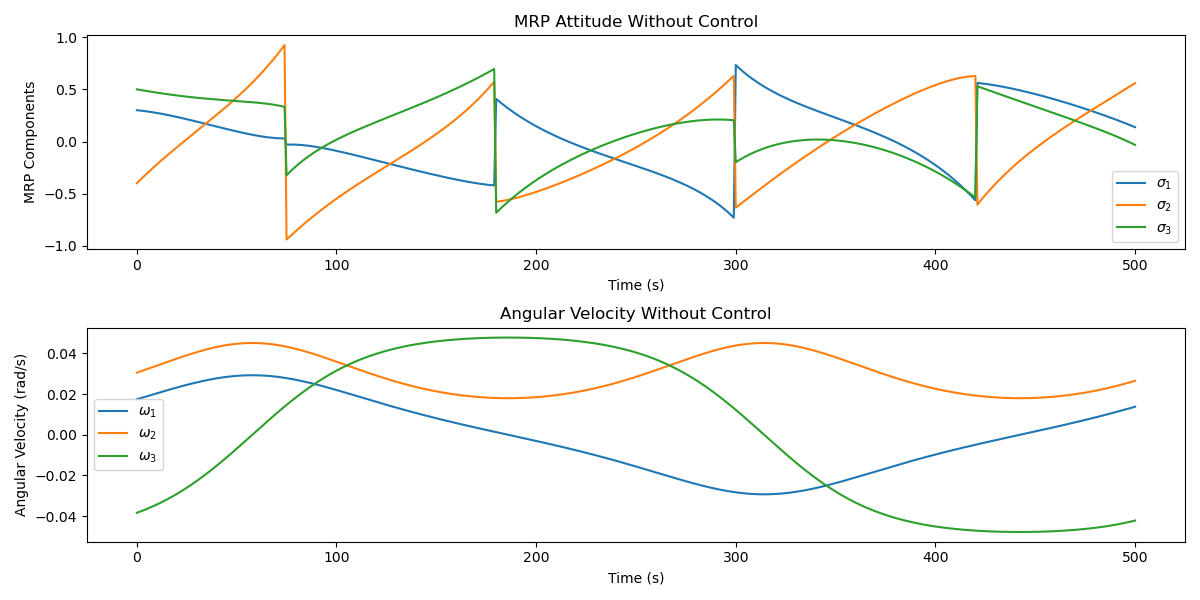
\includegraphics[width=1\linewidth]{task7_without_control.png}
    \caption{Attitude and angular velocity of our 500s simulation without control torque}
    \label{fig:enter-label}
\end{figure}
In Fig.4 we can see the MRPs evolve smoothly with periodic sharp transitions – this is the shadow set switching of MRPs to avoid singularities. This behavior is expected and shows the system rotating naturally without a control torque. Meanwhile, the angular velocity values exhibit an expected smooth oscillatory behavior. No component stays constant, which is typical for a free rigid body rotation with asymmetric inertia and no control torque.

Next we look at kinetic energy:
\begin{figure}[H]
    \centering
    \captionsetup{width=.7\linewidth}
    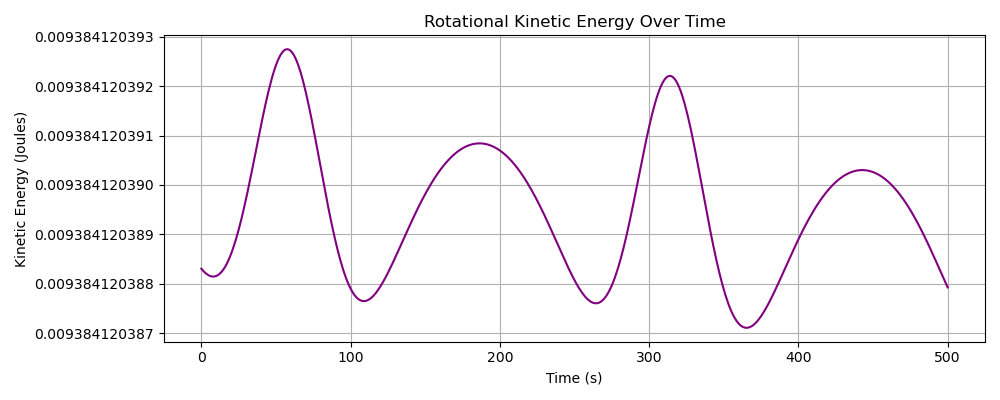
\includegraphics[width=1\linewidth]{task7_kinetic_energy.png}
    \caption{Kinetic Energy T of our spacecraft over 500s simulation without control torque}
    \label{fig:enter-label}
\end{figure}
In Fig.5, we see the rotational kinetic energy is almost perfectly constant, with only minor numerical fluctuations (on the order of $\num{1e-13}$). This further confirms that the system is torque-free, since no energy is being added or removed.

Next we plot both of the angular momentum vectors together to compare:
\begin{figure}[H]
    \centering
    \captionsetup{width=.7\linewidth}
    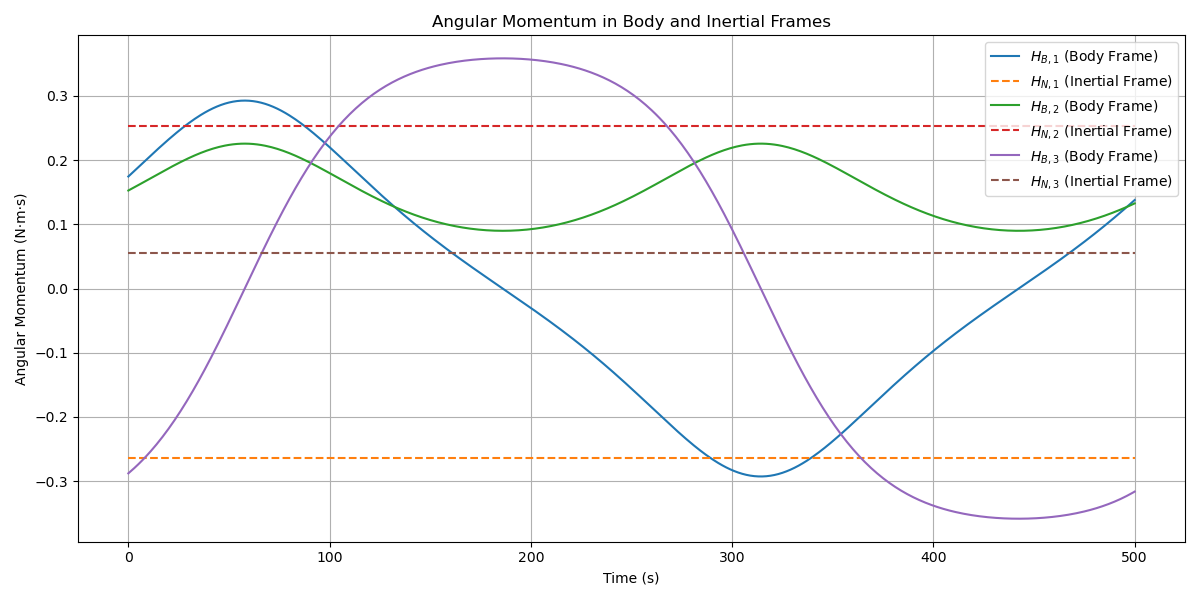
\includegraphics[width=1\linewidth]{task7_angular_momentum.png}
    \caption{Angular momentum of our spacecraft in inertial and body fixed frames over 500s simulation without control torque}
    \label{fig:enter-label}
\end{figure}
The angular momentum vector in the body frame ${}^B\mathbf{H}$ clearly changes over time, which is expected since the body frame is rotating. The angular momentum in the inertial frame ${}^N\mathbf{H}$ remains constant (flat dotted lines) throughout the entire simulation. This confirms conservation of angular momentum in an inertial frame when no external torques act on the system.

In summary, we can see that in the absence of external torques, the spacecraft demonstrates classic free rigid body dynamics. Angular momentum is conserved in the inertial frame, while its components in the rotating body frame vary over time. The rotational kinetic energy remains essentially constant, reinforcing the system's energy conservation. Looking at the attitude, the MRP evolution shows smooth lines except for the expected shadow set behavior, and angular velocities oscillate, all consistent with torque-free motion of an asymmetric rigid body.

Next we perform our analysis with a control torque ${}^B\bm u = (0.01, -0.01, 0.02)$ Nm. The logic is mostly the same, leveraging our RK4 inegrator while iterating over the simulation time from 0-100 seconds. During this simulation, we only save the history of the attitude and angular velocity. We can see the results below:
\begin{figure}[H]
    \centering
    \captionsetup{width=.7\linewidth}
    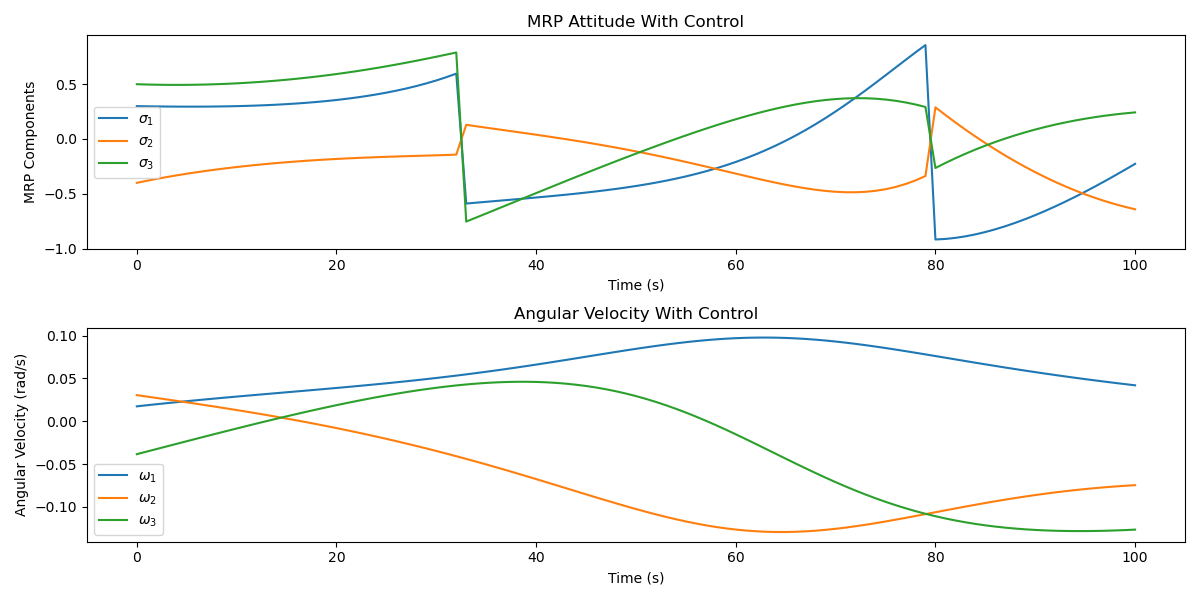
\includegraphics[width=1\linewidth]{task7_with_control.png}
    \caption{Attitude and angular velocity of our 100s simulation with control torque}
    \label{fig:enter-label}
\end{figure}
In this simulation we expect that the control torque is driving attitude changes more rapidly, which is evident in Fig.7 by the shadow set switching almost twice as frequently than in the un-controlled simulation. This more rapid orientation is a direct effect of the control torque actively rotating the spacecraft toward a desired state, as opposed to the more passive, natural motion observed in the torque-free case. Additionally, The angular velocity exhibits slightly more damped behavior, in contrast to the sustained oscillations seen without control. Over the 100-second period, the angular rates trend toward more steady values, confirming that the control input is successfully regulating rotational motion.

While these plots allow us to analyze the simulation, we are also tasked with providing their specific values at $t=500$. Doing so gives the following results:

\textbf{MRP Attitude,} $\bm{\sigma}_{B/N}(500\,\text{s})$:
\[
\begin{bmatrix}
\phantom{-}0.1377 \\
\phantom{-}0.5603 \\
-0.0322
\end{bmatrix}
\]

\textbf{Angular Momentum in Body Frame,} ${}^B\mathbf{H}(500\,\text{s})\ (\text{kg}\cdot\text{m}^2/\text{s})$:
\[
\begin{bmatrix}
\phantom{-}0.1379 \\
\phantom{-}0.1327 \\
-0.3164
\end{bmatrix}
\]

\textbf{Angular Momentum in Inertial Frame,} ${}^N\mathbf{H}(500\,\text{s})\ (\text{kg}\cdot\text{m}^2/\text{s})$:
\[
\begin{bmatrix}
-0.2641 \\
\phantom{-}0.2528 \\
\phantom{-}0.0553
\end{bmatrix}
\]

\textbf{Rotational Kinetic Energy,} $T(500\,\text{s})$:
\[
0.0094\ \text{J}
\]

\vspace{1em}
Next we do the same for our attitude at $t=100s$ for our simulation with the control torque added:

\textbf{MRP Attitude,} $\bm{\sigma}_{B/N}(100\,\text{s})$:
\[
\begin{bmatrix}
-0.2269 \\
-0.6414 \\
\phantom{-}0.2425
\end{bmatrix}
\]

Finally, we plug in these results to Coursera and see that our simulations and derivations are all working correctly.











\section{Task 8: Sun Pointing Control}
In the next few sections, well be testing each control pointing mode individually, with our final control torque incorporated, and then finally combine them all in the final task. For Task 8, we develop a simple PD control as shown in the following equation which was provided to us:
\[
{}^B\bm{u} = -K\bm{\sigma}_{B/R} - P{}^B\bm{\omega}_{B/R}
\]
For the next three tasks, we assume the spacecraft engages with the corresponding pointing control mode at time $t=0$. For all remaining tasks, we must integrate the control torque equation into our simulation, ensuring that our desired pointing is achieved with closed-loop performance. In this task, that desired pointing is the sun-pointing mode. We want to use linearized closed loop dynamics to determine the scalar attitude feedback gain $K$ and scalar angular velocity feedback gain $P$ such that the slowest decay response time is 120 seconds. Additionally, the closed loop response for all attitude components should be either critically damped or underdamped. This means our damping ratio must be $\xi\leq1$. From that information, we can start by deriving our $P$ value using the time decay equation
\[
T_i=\frac{2I_i}{P_i} \Longrightarrow P_i=\frac{2I_i}{T_i} \tag{\cite{schaub},~eq. 8.119}
\]
In this equation, we want $I_i$ to be the maximum inertia in our inertia tensor $[I]$ since the value of $T_i$ is maximized when $I$ is maximized. Since 120 seconds is our maximum decay time, we want to chose $I_{max}=10 \text{ kg m\textsuperscript{2}}$ to ensure that $T_i\leq120$s. Plugging this in yields
\[
P_i = \frac{2(10)}{120} = \frac{20}{120} = \frac{1}{6} = 0.1\overline{6}\quad \text{kg m\textsuperscript{2}/s}
\]
In a similar fashion we use this result to derive our value for $K$
\[
\xi_i=\frac{P_i}{\sqrt{KI_i}} \Longrightarrow \sqrt{KI_i}=\frac{P_i}{\xi_i} \Longrightarrow KI_i=\frac{{P_i}^2}{{\xi_i}^2} \Longrightarrow K=\frac{{P_i}^2}{{\xi_i}^2I_i} \tag{\cite{schaub},~eq. 8.118}
\]
Here, we want $I_i$ to be the minimum inertia in our inertia tensor $[I]$ since the value of $\xi_i$ is maximized when $I$ is minimized. Since $\xi\leq1$ is our maximum damping ratio, we want to chose $I_{min}=5 \text{ kg m\textsuperscript{2}}$ to ensure that $\xi\leq1$. Plugging in this along with our calculated value of $P$ yields
\[
K = \frac{{(\frac{1}{6})}^2}{1^2(5)} = \frac{\frac{1}{36}}{5} = \frac{1}{180} = 0.00\overline{5} \quad \text{kg m\textsuperscript{2}/s\textsuperscript{2}}
\]

Now that we have chosen our values for $K$ and $P$, we can write a function to compute our control torque ${}^B\bm u$. This function is called \texttt{PD\_controller(t, sigma\_bn, omega\_bn, RN, omega\_rn, K, P)}. It computes the current control torque vector ${}^B\bm u$ as defined in the equation above. To do this, it first has to call our function from Task 6, \texttt{getTrackingErrors}. Recall that this function returns the two values needed to compute ${}^B\bm u,\ \bm\sigma_{B/R}$ and ${}^B\bm\omega_{B/R}$. A full description is given in Task 6. The main thing to note here is that for Task 8, the \texttt{PD\_controller} DCM $[RN]$ is the sun-pointing DCM $[R_sN]$ and the value passed as \texttt{omega\_rn} is ${}^N\bm\omega_{R_s/N}$. After obtaining these values, the control torque is computed and returned by simply plugging in all of our values. 

We can now start our simulation loop, similarly to how we completed Task 7. This time, we run the simulation for $t=500$s. We iterate through each timestep, saving both $\bm\sigma_{B/N}$ and ${}^B\bm\omega_{B/N}$ for plotting and calling our RK4 integrator with the \texttt{dynamics} function from Task 7. Each iteration, we update the value of the control torque ${}^B\bm u$ before passing it to the integrator. Note that as said earlier in the report, we are always checking for the shadow set condition in all of these simulations. 

Finally, we can view our results:
\begin{figure}[H]
    \centering
    \captionsetup{width=.7\linewidth}
    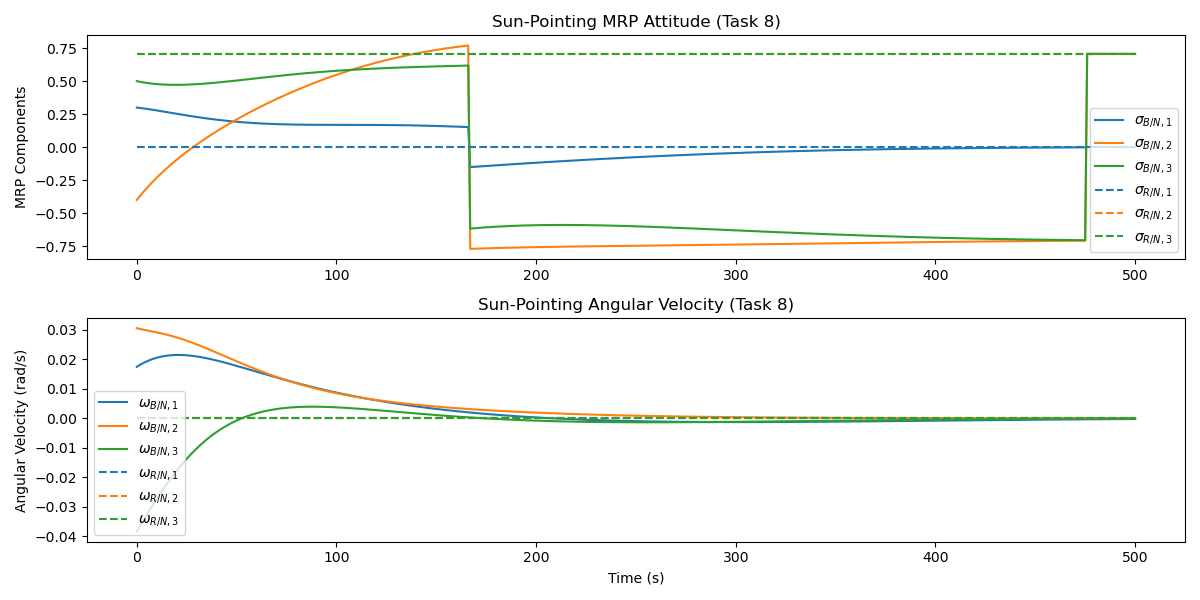
\includegraphics[width=1\linewidth]{task8_sun_pointing_control.png}
    \caption{Attitude and angular velocity plotted against their reference values for a 500s simulation of our control torque driving the craft to the sun-pointing reference frame.}
    \label{fig:enter-label}
\end{figure}
In this simulation we see the attitudes and velocities being driven to their reference values (dotted lines) as expected. Here, the attitudes are constant straight lines since, as we found Task 3, the sun pointing reference from is not a function of time. However, something interesting is also happening here. If a closer look is taken at the MRPs, it can be observed that they actually flip to being driven to their shadow set version of the reference frame at \textasciitilde180 seconds. Looking into this, we investigate the sun-pointing reference frame defined in Task 3 to find that its MRP equivalent is 
\[
\bm{\sigma}_{R_s/N} =
\begin{bmatrix}
0 \\ 0.70710678 \\ 0.70710678
\end{bmatrix}
\]
Taking the magnitude of this MRP set gives us $|\bm\sigma| = 0.99999999664$. Considering that the shadow set threshold for the norm is exactly 1, we see that we are only a few billionths of a decimal off from switching to the shadow set for this reference frame attitude set. This explains the odd behavior in the plot. Basically, as the spacecraft is being driven to the shadow set threshold, tiny numerical errors on the order of $\num{1e-9}$ cause the attitude representation to flip sets. We can see further down the simulation it flips back to the reference value. This will likely continuously occur if we extend our simulation. Remember that this is just the representation of the attitude state. Since these flips do not signify the spacecraft undergoing any significant rotation, these are a perfectly fine anomaly to see in our plots. Furthermore, if it was desired, we could even mitigate this effect by adjusting our shadow set threshold from its current value of 1, to a number slightly larger than 1 e.g. 1 + \num{1e-7}. This should keep other results mostly the same, while not allowing this particular case to flip back and forth since the numerical precision error that would cause shadow set flipping on this attitude set is on an order that is smaller than \num{1e-7}.

Looking at the angular velocity values, we can see they are all driven to 0, which is what we expect for the the sun-pointing frame. Here, the green dotted line is the only reference line shown, since all the reference values for angular velocity are exactly 0 in this case.

Next, we are tasked with providing specific MRP values at various time steps. Doing so gives the following results:

$\bm{\sigma}_{B/N}(15\,\text{s})$:
\[
\begin{bmatrix}
\phantom{-}0.2656 \\
-0.1598 \\
\phantom{-}0.4733
\end{bmatrix}
\]

$\bm{\sigma}_{B/N}(100\,\text{s})$:
\[
\begin{bmatrix}
\phantom{-}0.1688 \\
\phantom{-}0.5482 \\
\phantom{-}0.5789
\end{bmatrix}
\]

$\bm{\sigma}_{B/N}(200\,\text{s})$:
\[
\begin{bmatrix}
-0.1181 \\
-0.7579 \\
-0.5915
\end{bmatrix}
\]

$\bm{\sigma}_{B/N}(400\,\text{s})$:
\[
\begin{bmatrix}
-0.0101 \\
-0.7188 \\
-0.6861
\end{bmatrix}
\]

\vspace{1em}
Finally, we plug in these results to Coursera and see that our simulations and derivations are all working correctly.







\section{Task 9: Nadir Pointing Control}
The next two tasks, including this one, are very similar to Task 8. We do the exact same process we did there, but are now running the simulation for the remaining two reference frames. Here, we will simulate the nadir-pointing frame $\mathcal{R}_n$. Our $K$ and $P$ values have already been derived, and we use them again here, and for the remainder of the assignment. We also keep our PD control the same as well. 

We start our simulation loop again, saving states and rates and calling the RK4 integrator. The main difference for this task is that the \texttt{PD\_controller} DCM $[RN]$ is the nadir-pointing DCM $[R_nN]$ and the value passed as \texttt{omega\_rn} is ${}^N\bm\omega_{R_n/N}$.
Afterwards, we can plot our results:
\begin{figure}[H]
    \centering
    \captionsetup{width=.7\linewidth}
    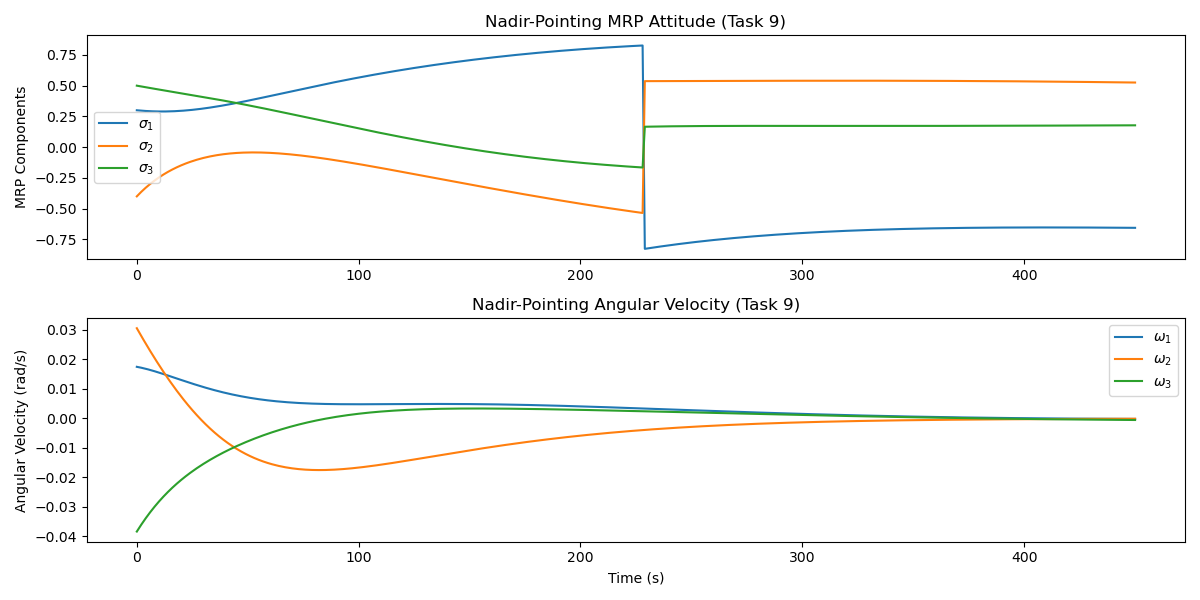
\includegraphics[width=1\linewidth]{task9_nadir_pointing_control.png}
    \caption{Attitude and angular velocity plotted against their reference values for a 500s simulation of our control torque driving the craft to the Nadir-pointing reference frame.}
    \label{fig:enter-label}
\end{figure}

These plots are in line with all of our expectations. We can see the attitude being driven to its reference value, and the angular velocities being driven to their near 0 reference values as well. Clearly our control torque is working correctly. Note that while the attitudes look flat, they have a very subtle slope/curvature to them. This contrasts with the actual flat lines seen in the sun-pointing analysis. This is expected as the attitude should be changing very slowly over time, indirectly proportional to the LMO's orbital period for nadir-pointing. This also explains why the angular velocities are near 0, since we are rotating at a relatively slow rate. If you look closely, you can see the reference velocities have small fluctuations around 0 rad/s, as expected.
We can also observe some noticeable under-damping in the ${}^B\omega_2$ value. This is expected since this is about the axis of least inertia for our spacecraft. This is fine since we are still meeting our control law requirement of being critically damped or under-damped.

We are also tasked with providing specific MRP values for this task. We need the values at the same time-steps as Task 8. The results are as follows:

$\bm{\sigma}_{B/N}(15\,\text{s})$:
\[
\begin{bmatrix}
\phantom{-}0.2911 \\
-0.1912 \\
\phantom{-}0.4535
\end{bmatrix}
\]

$\bm{\sigma}_{B/N}(100\,\text{s})$:
\[
\begin{bmatrix}
\phantom{-}0.5661 \\
-0.1374 \\
\phantom{-}0.1522
\end{bmatrix}
\]

$\bm{\sigma}_{B/N}(200\,\text{s})$:
\[
\begin{bmatrix}
\phantom{-}0.7958 \\
-0.4598 \\
-0.1265
\end{bmatrix}
\]

$\bm{\sigma}_{B/N}(400\,\text{s})$:
\[
\begin{bmatrix}
-0.6528 \\
\phantom{-}0.5349 \\
\phantom{-}0.1746
\end{bmatrix}
\]

Again, we plug these into Coursera and confirm everything is working as expected.

\section{Task 10: GMO Pointing Control}
For this task, we complete the reference frame simulations with the GMO/Communication reference frame $\mathcal{R}_c$. The same details regarding control torque and simulation parameters that were discussed in Tasks 8 and 9 also apply here. Again, the only difference for this task is that for the \texttt{PD\_controller} function, the DCM $[RN]$ is the GMO-pointing DCM $[R_cN]$ and the value passed as \texttt{omega\_rn} is ${}^N\bm\omega_{R_c/N}$. Using this, we start our simulation and save our state and rates for each time step, the same as before. 

Afterwards, we plot our results:
\begin{figure}[H]
    \centering
    \captionsetup{width=.7\linewidth}
    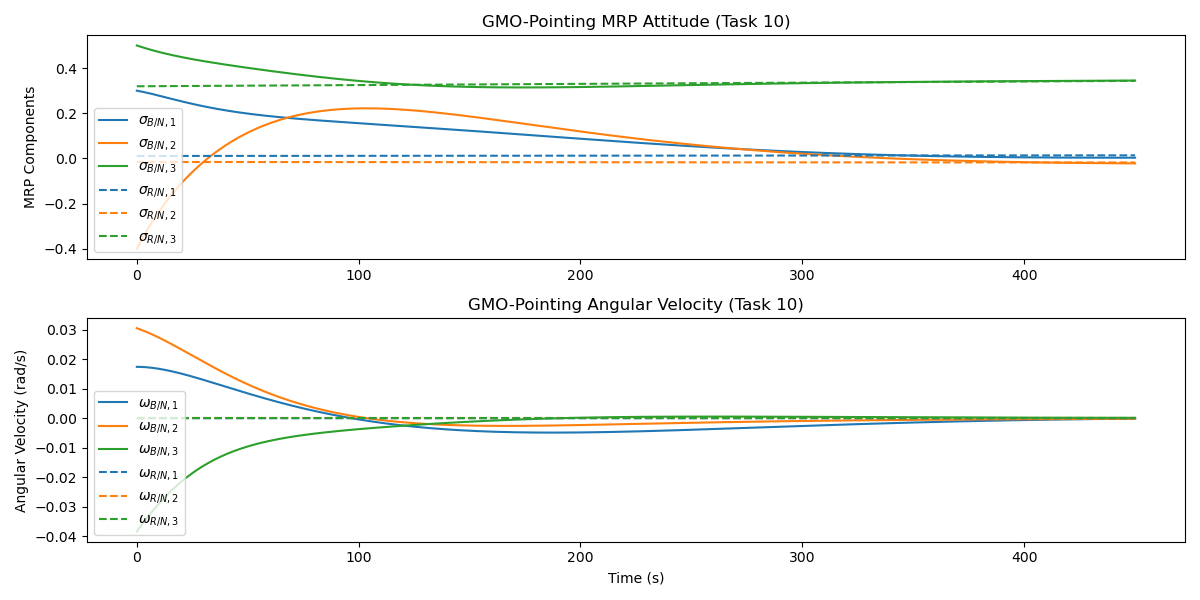
\includegraphics[width=1\linewidth]{task10_gmo_pointing_control.png}
    \caption{Attitude and angular velocity plotted against their reference values for a 500s simulation of our control torque driving the craft to the GMO-pointing reference frame.}
    \label{fig:enter-label}
\end{figure}
Here, we see similar results to Tasks 8 and 9. The states and rates are driven to their reference values. We can observe some noticeable under-damping in the $\sigma_2$ component which is acceptable. The angular velocity values are all minimally under-damped and very close to critical damping. Similarly to Task 9, the reference attitudes appear flat, but do have a measurable slope/curvature. Since we are GMO pointing, the reference value rates are indirectly proportional to both the LMO and GMO orbital periods. The same is true for the angular velocities. They are near 0 since we are rotating slowly, but do have real values that are changing over time.

Last, we are tasked with providing specific MRP values at various time steps. Doing so gives the following results:

$\bm{\sigma}_{B/N}(15\,\text{s})$:
\[
\begin{bmatrix}
\phantom{-}0.2654 \\
-0.1688 \\
\phantom{-}0.4595
\end{bmatrix}
\]

$\bm{\sigma}_{B/N}(100\,\text{s})$:
\[
\begin{bmatrix}
\phantom{-}0.1561 \\
\phantom{-}0.2216 \\
\phantom{-}0.3432
\end{bmatrix}
\]

$\bm{\sigma}_{B/N}(200\,\text{s})$:
\[
\begin{bmatrix}
\phantom{-}0.0873 \\
\phantom{-}0.1193 \\
\phantom{-}0.3162
\end{bmatrix}
\]

$\bm{\sigma}_{B/N}(400\,\text{s})$:
\[
\begin{bmatrix}
\phantom{-}0.0050 \\
-0.0165 \\
\phantom{-}0.3424
\end{bmatrix}
\]

Finally, we plug in these results to Coursera and see that our simulations and derivations are all working correctly.

\section{Task 11: Mission Scenario Simulation}

Finally we arrive at our final task: full mission scenario simulation. 

This task differs from the previous 3 in that we are finally going to control the mode switching of the spacecraft during our simulation loop. In previous tasks, we assumed a single reference frame (or no reference in Task 7) and stayed with it for the entire duration of the simulation. Here, we need to implement logic to switch reference frames when certain criteria are met. When that happens, the the DCM $[RN]$ and \texttt{omega\_rn} values for the \texttt{PD\_controller} function are updated to the new reference frame. This allows our control law to always drive us to our currently desired reference frame. 

To implement these mode-switching criteria, we can look back to Table \ref{table1} from the Introduction. This gives an overview of the control logic. We will write a function called \texttt{determine\_control\_mode(r\_LMO\_inertial, r\_GMO\_inertial)} to implement this logic. The two arguments represent the positional vectors of each spacecraft, ${}^N\bm r_{LMO}$ and ${}^N\bm r_{GMO}$. To get these two vectors, we of course use our function from Task 1, \texttt{getInertialPositionVectors}, which was written to do this exact task. For a full description, refer to Task 1. Once we get both position vectors returned, we are ready to call our \texttt{determine\_control\_mode} function. Now we just need to figure out how it should work. 

Looking at the table, we see that if the satellite is on the sunlit side of Mars, it will always be charging. To check this, we need the ${}^N\bm r_{LMO}$ vector. Since this vector is expressed with $\mathcal{N}$ frame components, all we need to do here is check if the second ($\hat{\bm n}_2$) component of the vector is $>0$. If it is, we are guaranteed to be in charging mode, and our reference frame $\mathcal{R}$ will be the sun-pointing frame $\mathcal{R}_s$. 

If this check fails, we we know we are on the dark side of Mars. Here, we always want to first attempt communication with the GMO satellite, but only if we are within our 35\textdegree\ angular difference threshold for communication with the GMO satellite. To check this, we need both the ${}^N\bm r_{LMO}$ and ${}^N\bm r_{GMO}$ vectors. We know that
\[
\cos(\theta) = \frac{{}^N\bm r_{LMO}\cdot{}^N\bm r_{GMO}}{|{}^N\bm r_{LMO}|\ |{}^N\bm r_{GMO}|}
\]
Here, $\theta$ is the angle between the two satellite position vectors. Since we have all the information for the right hand side of the equation, we simply take the $\arccos$ to solve for the angle $\theta$. We then check if $\theta < 35\textdegree$. If it is, we will be in communication mode and our reference frame $\mathcal{R}$ will be the GMO-pointing frame $\mathcal{R}_c$.

If neither of these criteria are met, then we know we are on the dark side of Mars and out of range for communication with GMO. If this is the case, we default to pointing our sensors in the nadir direction to get science data from Mars' surface. This means our reference frame $\mathcal{R}$ will be the nadir-pointing frame $\mathcal{R}_n$.

We implement these criteria with an \texttt{if-else} block in our function, giving us the logic needed for switching control modes of the LMO satellite. Finally, our \texttt{determine\_control\_mode} function is ready. 

We start our simulation and save our state and rates for each time step, the same as before. This time, we are simulating for 6500 seconds. Remember, we do everything the same as before, the only difference for this task is we are switching the reference frame DCM $[RN]$ and \texttt{omega\_rn} values for the \texttt{PD\_controller}.

Afterwards, we plot our results:
\begin{figure}[H]
    \centering
    \captionsetup{width=.7\linewidth}
    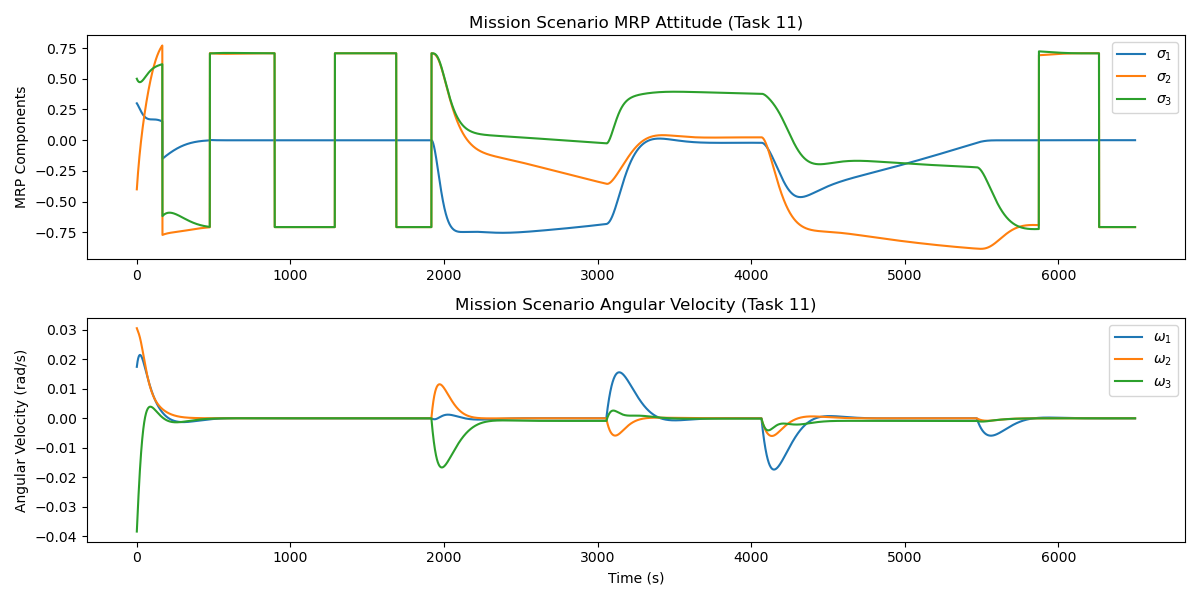
\includegraphics[width=1\linewidth]{task11_mission_scenario.png}
    \caption{Attitude and angular velocity plotted against their reference values for a 6500s simulation of our control torque driving the craft to the varying reference frames detailed in our mission.}
    \label{fig:enter-label}
\end{figure}
Looking at this figure gives interesting, but expected, results. Comparing to the figures presented in Tasks 8-10, we can identify each of the modes. We start in the sun-pointing mode, and undergo a total of 4 control mode changes during our 6500s mission simulation time. The control mode changes are evident in both plots, but each mode change is most obviously distinguishable in the angular velocity chart. Each blip in the plot represents our control torque changing, and shows how our satellite is re-orienting into the next reference frame.

The first mode change can be seen at \textasciitilde2000 seconds. Looking back at the plots in the previous tasks, we see this is to the nadir reference frame. Here, we can finally see the slopes in the attitudes that have been discussed previously. This is because we are running a longer simulation and thus have a zoomed out view. 

At just over \textasciitilde3000 seconds, we see our second mode change. Again, this can be confirmed as the GMO-pointing mode. We can see the reference MRP values match those of our Task 10 plot perfectly. The MRP slope/rate of change is very subtle here, which aligns with our results in Task 5, which determined that the angular velocity values of the GMO-pointing frame were very small, on the order of \num{1e-5} rad/s.

At roughly \textasciitilde4000 seconds, we see our third switch. This time we can tell is is going back to the nadir-pointing reference. We can observe how in both of the nadir modes in the plot, the attitudes have a sharper slopes compared to GMO mode, which aligns with our results for the nadir mode angular velocity values from Task 4 as well. 

Finally, we have our final mode switch, back to sun-pointing mode, at \textasciitilde5500 seconds. In both this instance and in the sun-pointing instance at the beginning of the simulation, we can see the MRP shadow set switching discussed extensively in Task 9. This helps further confirm what mode we are looking for these two segments of the simulation. The spacecraft appears to stay in this mode until 6500 seconds, when our simulation ends. 

All of these findings and discussions also help explain the angular velocity plot seen on the bottom. For this plot, we can see the perfectly 0 (green) reference values for both of the sun-pointing modes. When we switch to the nadir modes, we see disturbances and fluctuations in the reference velocity values, confirming our small but non 0 values calculated during previous simulations. Finally, for the GMO-pointing mode, we see nearly invisible fluctuations, but are just able to make out the switching of the green and orange color on the plot. 

Our last observation concerns the damping. Looking at the plot, we see successful under- or critical damping for all mode switching across every axis of the spacecraft. The values are driven to their reference values, but don't exhibit over-damped behavior or any highly visible under-damping. This is exactly what we designed our control law to do, confirming that our simulation implementation is working correctly. 

For our final requirement, we are tasked with providing specific MRP values at various time steps. Doing so gives the following results:

$\bm{\sigma}_{B/N}(300\,\text{s})$:
\[
\begin{bmatrix}
-0.0442 \\
-0.7386 \\
-0.6307
\end{bmatrix}
\]

$\bm{\sigma}_{B/N}(2100\,\text{s})$:
\[
\begin{bmatrix}
-0.7458 \\
\phantom{-}0.1139 \\
\phantom{-}0.1581
\end{bmatrix}
\]

$\bm{\sigma}_{B/N}(3400\,\text{s})$:
\[
\begin{bmatrix}
\phantom{-}0.0132 \\
\phantom{-}0.0398 \\
\phantom{-}0.3907
\end{bmatrix}
\]

$\bm{\sigma}_{B/N}(4400\,\text{s})$:
\[
\begin{bmatrix}
-0.4331 \\
-0.7323 \\
-0.1877
\end{bmatrix}
\]

$\bm{\sigma}_{B/N}(5600\,\text{s})$:
\[
\begin{bmatrix}
-0.0012 \\
-0.8260 \\
-0.5044
\end{bmatrix}
\]

Finally, we plug in these results to Coursera and see that our simulations and derivations are all working correctly.

\section{Conclusion}
This report presents the complete development and analysis of a nano-satellite’s attitude dynamics and control system in a Mars-centered orbit. Through Tasks 1–11, we designed, implemented, and verified a comprehensive simulation framework capable of modeling the satellite’s behavior across multiple mission modes—science, charging, and communication. 

Starting with orbital mechanics, we derived inertial positions and velocities from orbital elements and constructed key reference frames including sun-pointing, nadir-pointing, and GMO-pointing attitudes. By leveraging modified Rodrigues parameters (MRPs) and associated angular velocity vectors, we were able to represent spacecraft attitude robustly while accounting for shadow set switching to avoid singularities.

A custom Runge-Kutta 4 integrator was implemented to propagate both attitude and angular velocity over time, and we developed a PD control law that stabilized the spacecraft orientation with respect to changing reference frames. Simulation results from Tasks 7 through 11 demonstrated the dynamic response of the spacecraft under both uncontrolled and controlled conditions. The controller was successfully tuned to achieve critical or under-damped performance while satisfying specified decay times and mode-switching criteria.

In the final mission scenario, the spacecraft responded appropriately to environmental and positional cues, autonomously switching between operational modes. Our results showed effective convergence to reference frames, minimal overshoot, and accurate long-duration tracking—all validated both visually through plots and quantitatively by extracting and verifying state values at specific time steps.

Overall, this project provided valuable hands-on experience in space vehicle dynamics, attitude control, and reference frame logic. The combination of analytical derivations, numerical methods, and simulation-based validation offers a rigorous and realistic demonstration of how modern spacecraft achieve precise orientation and reconfiguration in planetary orbits.

\section*{Appendix}
\section*{A. Code Listing}
\addcontentsline{toc}{section}{A. Code Listing}
\begin{pythoncode}
import numpy as np
from sympy import symbols, pprint, cos, sin, Matrix, pi
import sympy as sp
import matplotlib.pyplot as plt

############################## Welcome ##############################
print("Welcome to the ASEN 5010 Capstone Project")
print("Attitude Dynamics and Control of a Nano-Satellite Orbiting Mars")

############################## Initial state ##############################
h = 400  # km
R_mars = 3396.19  # km
r_lmo = R_mars + h
mu = 42828.3  # km^3/s^2
theta_lmo_rate = 0.000884797  # rad/s
mars_period_min = (24 * 60) + 37
mars_period_sec = mars_period_min * 60
mars_period_hr = mars_period_min / 60
gmo_period_sec = mars_period_sec
r_gmo = 20424.2  # km
theta_gmo_rate = 0.0000709003  # rad/s
tmax = 6500  # Set the value of tmax
dt = 0.1  # Set the value of Δt
t_0 = 0.0  # Initial time
sigma_bn_0 = np.array([0.3, -0.4, 0.5])  # MRPs
omega_bn_0 = np.array([1.00, 1.75, -2.20])  # deg/s
omega_bn_0_rad = np.deg2rad(omega_bn_0)
I_b = np.array([[10, 0, 0], [0, 5, 0], [0, 0, 7.5]])  # kg*m^2
I_b_inv = np.linalg.inv(I_b)
X_0 = np.concatenate((sigma_bn_0, omega_bn_0_rad))  # Initial conditions
omega_lmo_0 = np.deg2rad(20)
i_lmo_0 = np.deg2rad(30)
theta_lmo_0 = np.deg2rad(60)  # function of time
omega_gmo_0 = 0
i_gmo_0 = 0
theta_gmo_0 = np.deg2rad(250)  # function of time
comm_angle_threshold = 35  # deg


############################## Helper Functions ##############################
def writeToFile(path, data):
    str_to_write = ""

    # Convert scalar to list
    if np.isscalar(data):
        str_to_write = str(data)
    else:
        if data.ndim == 2:
            for row in data:
                for element in row:
                    str_to_write += str(element) + " "
        else:
            for element in data:
                str_to_write += str(element) + " "
    with open(path, "w+") as file:
        file.write(str_to_write.rstrip())


def theta_lmo(t):
    return theta_lmo_0 + t * theta_lmo_rate


def theta_gmo(t):
    return theta_gmo_0 + t * theta_gmo_rate


def s(theta):
    return np.sin(theta)


def c(theta):
    return np.cos(theta)


# Returns a skew-symmetric matrix from a vector
def tilde(v):
    return np.array([[0, -v[2], v[1]], [v[2], 0, -v[0]], [-v[1], v[0], 0]])


def Euler313toDCM(t1, t2, t3):
    # Convert 313 angles to DCM - From appendix B.1
    return np.array(
        [
            [
                c(t3) * c(t1) - s(t3) * c(t2) * s(t1),
                c(t3) * s(t1) + s(t3) * c(t2) * c(t1),
                s(t3) * s(t2),
            ],
            [
                -s(t3) * c(t1) - c(t3) * c(t2) * s(t1),
                -s(t3) * s(t1) + c(t3) * c(t2) * c(t1),
                c(t3) * s(t2),
            ],
            [s(t2) * s(t1), -s(t2) * c(t1), c(t2)],
        ]
    )


def DCM2Quaternion(C):
    # Initialize stuff
    B = np.zeros(4)  # B^2 array
    b = np.zeros(4)  # resulting set of quaternions
    trc = np.trace(C)

    B[0] = (1 + trc) / 4
    B[1] = (1 + 2 * C[0, 0] - trc) / 4
    B[2] = (1 + 2 * C[1, 1] - trc) / 4
    B[3] = (1 + 2 * C[2, 2] - trc) / 4

    # Find the index of the maximum value in B2
    i = np.argmax(B)

    # Calculate quaternion based on sheppard's method
    if i == 0:
        b[0] = np.sqrt(B[0])
        b[1] = (C[1, 2] - C[2, 1]) / (4 * b[0])
        b[2] = (C[2, 0] - C[0, 2]) / (4 * b[0])
        b[3] = (C[0, 1] - C[1, 0]) / (4 * b[0])
    elif i == 1:
        b[1] = np.sqrt(B[1])
        b[0] = (C[1, 2] - C[2, 1]) / (4 * b[1])
        if b[0] < 0:
            b[1] = -b[1]
            b[0] = -b[0]
        b[2] = (C[0, 1] + C[1, 0]) / (4 * b[1])
        b[3] = (C[2, 0] + C[0, 2]) / (4 * b[1])
    elif i == 2:
        b[2] = np.sqrt(B[2])
        b[0] = (C[2, 0] - C[0, 2]) / (4 * b[2])
        if b[0] < 0:
            b[2] = -b[2]
            b[0] = -b[0]
        b[1] = (C[0, 1] + C[1, 0]) / (4 * b[2])
        b[3] = (C[1, 2] + C[2, 1]) / (4 * b[2])
    elif i == 3:
        b[3] = np.sqrt(B[3])
        b[0] = (C[0, 1] - C[1, 0]) / (4 * b[3])
        if b[0] < 0:
            b[3] = -b[3]
            b[0] = -b[0]
        b[1] = (C[2, 0] + C[0, 2]) / (4 * b[3])
        b[2] = (C[1, 2] + C[2, 1]) / (4 * b[3])

    return b


def MRP2DCM(sigma):
    tilde_sigma = tilde(sigma)
    return np.eye(3) + (
        8 * tilde_sigma @ tilde_sigma - 4 * (1 - sigma @ sigma) * tilde_sigma
    ) / ((1 + sigma @ sigma) ** 2)


def checkShadowSet(sigma):
    if np.linalg.norm(sigma) > 1:
        return -sigma / (sigma @ sigma)
    else:
        return sigma


def DCM2MRP(C):
    b = DCM2Quaternion(C)
    divisor = 1 + b[0]
    sigma = np.array([b[1], b[2], b[3]]) / divisor
    return checkShadowSet(sigma)


############################## Task 1: Orbit Simulation (5 points) ##############################
# pos = r*i_r
# Derive inertial s/c velocity r_dot.
# Note that for circular orbits, theta_dot is constant
print("\n\nBEGIN TASK 1")


# Write a function whose inputs are radius r and 313 angles omega, i, theta,
# and outputs are the inertial pos vector N_r and vel N_r_dot
# Calculate the inertial position vector N_r and velocity N_r_dot
def getInertialPositionVectors(r, omega, i, theta):
    # O : {i_r, i_theta, i_h} aka H frame
    # N : {n_1, n_2, n_3}
    ON = Euler313toDCM(omega, i, theta)
    NO = ON.T
    # Convert direction of i_r to N
    N_r = NO @ np.array([r, 0, 0])
    # Convert direction of i_theta to N
    if r == r_lmo:
        N_r_dot = NO @ np.array([0, r * theta_lmo_rate, 0])
    if r == r_gmo:
        N_r_dot = NO @ np.array([0, r * theta_gmo_rate, 0])
    return N_r, N_r_dot


# confirm the operation by checking getInertialVectors(r_lmo, omega_lmo, i_lmo, theta_lmo(450))
# and getInertialVectors(r_gmo, omega_gmo, i_gmo, theta_gmo(1150))
N_r_lmo, N_r_lmo_dot = getInertialPositionVectors(
    r_lmo, omega_lmo_0, i_lmo_0, theta_lmo(450)
)
N_r_gmo, N_r_gmo_dot = getInertialPositionVectors(
    r_gmo, omega_gmo_0, i_gmo_0, theta_gmo(1150)
)
print("rLMO = ", N_r_lmo)
print("vLMO = ", N_r_lmo_dot)
print("rGMO = ", N_r_gmo)
print("vGMO = ", N_r_gmo_dot)
writeToFile("./tasks/task 1/rLMO.txt", N_r_lmo)
writeToFile("./tasks/task 1/vLMO.txt", N_r_lmo_dot)
writeToFile("./tasks/task 1/rGMO.txt", N_r_gmo)
writeToFile("./tasks/task 1/vGMO.txt", N_r_gmo_dot)


############################## Task 2: Orbit Frame Orientation (5 points) ##############################
print("\n\nBEGIN TASK 2")
Omega, i = symbols("Omega i")
t = symbols("t", positive=True)
theta = sp.Function(symbols("theta"))
HN = Matrix(
    [
        [
            cos(theta(t)) * cos(Omega) - sin(theta(t)) * cos(i) * sin(Omega),
            cos(theta(t)) * sin(Omega) + sin(theta(t)) * cos(i) * cos(Omega),
            sin(theta(t)) * sin(i),
        ],
        [
            -sin(theta(t)) * cos(Omega) - cos(theta(t)) * cos(i) * sin(Omega),
            -sin(theta(t)) * sin(Omega) + cos(theta(t)) * cos(i) * cos(Omega),
            cos(theta(t)) * sin(i),
        ],
        [sin(i) * sin(Omega), -sin(i) * cos(Omega), cos(i)],
    ]
)
with open("./latex/task_2_HN.tex", "w+") as file:
    file.write((sp.latex(HN)))


# Write a function whose input is time t and output is DCM HN(t) for the LMO
def getHNforLMO(t):
    return Euler313toDCM(omega_lmo_0, i_lmo_0, theta_lmo(t))


# Validate the operation by computing HN(300)
t = 300  # sec
HN_at_t = getHNforLMO(t)
print("HN(t = " + str(t) + "s) = ", HN_at_t)
writeToFile("./tasks/task 2/HN.txt", HN_at_t)


############################## Task 3: Sun-Pointing Reference Frame Orientation (10 points) ##############################
print("\n\nBEGIN TASK 3")
# First determine and analytic expression for Rs by defining DCM [RsN]
RsN = np.array([[-1, 0, 0], [0, 0, 1], [0, 1, 0]])
with open("./latex/RsN.tex", "w+") as file:
    file.write((sp.latex(RsN)))


# Write a function that returns RsN
def getRsN():
    return RsN


def getOmegaRsN():
    return np.array([0, 0, 0])


# Validate the evalutation of RsN by providing numerical values for t=0s
print("RsN(t = 0s) = ", getRsN())
writeToFile("./tasks/task 3/RsN.txt", getRsN())

# Angular velocity is [0, 0, 0] since the DCM is not a function of time
print("N_ω_Rn/N = ", getOmegaRsN())
writeToFile("./tasks/task 3/omega_rs_n.txt", getOmegaRsN())


############################## Task 4: Nadir-Pointing Reference Frame Orientation (10 points) ##############################
print("\n\nBEGIN TASK 4")
# First determine and analytic expression for Rn by defining DCM [RnN]
RnH = np.array([[-1, 0, 0], [0, 1, 0], [0, 0, -1]])
with open("./latex/RnH.tex", "w+") as file:
    file.write((sp.latex(RnH)))
with open("./latex/RnN.tex", "w+") as file:
    file.write((sp.latex(RnH @ HN)))


# Write a function that returns RnN
def getRnN(t):
    return RnH @ getHNforLMO(t)


# Write a function that determines angular velocity vector omega_rn_n
def getOmegaRnN(t):
    NRn = getRnN(t).T
    return NRn @ [0, 0, -theta_lmo_rate]  # ω = θ_dot*i_h = -θ_dot*r_3


t = 330  # sec
# Validate the evalutation of RnN by providing numerical values for t = 330s
RnN_at_t = getRnN(t)
print("RnN(t = " + str(t) + "s) = ", RnN_at_t)
writeToFile("./tasks/task 4/RnN.txt", RnN_at_t)

# What is the angular velocity @ t = 330s
omega_rnn_at_t = getOmegaRnN(t)
print("N_ω_Rn/N(t = " + str(t) + "s) = ", omega_rnn_at_t)
writeToFile("./tasks/task 4/omega_rn_n.txt", omega_rnn_at_t)


############################## Task 5: GMO-Pointing Reference Frame Orientation (10 points) ##############################
print("\n\nBEGIN TASK 5")


# dr = r_gmo - r_lmo  => lets get these in N frame to make cross product easy
# H : {i_r, i_theta, i_h} - Note theres one for GMO, one for LMO, depending on theta
# N : {n_1, n_2, n_3}
# Write a function that returns RcN
def getRcNExpr():
    NH = HN.T
    theta_gmo_expr = sp.Function(symbols("theta_GMO"))
    theta_lmo_expr = sp.Function(symbols("theta_LMO"))
    NH_gmo = NH.subs([(Omega, omega_gmo_0), (i, i_gmo_0), (theta, theta_gmo_expr)])
    NH_lmo = NH.subs([(Omega, omega_lmo_0), (i, i_lmo_0), (theta, theta_lmo_expr)])
    N_r_gmo_col = NH_gmo @ sp.Matrix([r_gmo, 0, 0])
    N_r_lmo_col = NH_lmo @ sp.Matrix([r_lmo, 0, 0])

    N_dr_col = N_r_gmo_col - N_r_lmo_col
    N_r1_col = -N_dr_col.normalized()
    N_r2_col = (N_dr_col.cross(sp.Matrix([0, 0, 1]))).normalized()
    N_r3_col = N_r1_col.cross(N_r2_col).normalized()

    return (sp.Matrix.hstack(N_r1_col, N_r2_col, N_r3_col)).T


def getRcN(t):
    RcN = getRcNExpr()
    RcN_f = sp.lambdify(
        ["t"],
        RcN,
        modules=["numpy", {"theta_GMO": theta_gmo}, {"theta_LMO": theta_lmo}],
    )
    return RcN_f(t)


# Write a function that determines angular velocity vector omega_rc_n
def getOmegaRcNAnalytically(time):
    t = symbols("t", positive=True)
    RcN = getRcNExpr()
    # RcNT = RcN.T

    # Replace with base functions so sympy knows how to derive wrt t
    theta_gmo_expr = sp.Function(symbols("theta_GMO"))
    theta_lmo_expr = sp.Function(symbols("theta_LMO"))
    replace_gmo = theta_gmo_0 + t * theta_gmo_rate
    replace_lmo = theta_lmo_0 + t * theta_lmo_rate
    replace_dict = {theta_gmo_expr(t): replace_gmo, theta_lmo_expr(t): replace_lmo}
    RcN_rep = RcN.subs(replace_dict)

    # Now sympy can take derivative wrt t
    RcN_dot = sp.diff(RcN_rep, t)
    omega_tilde = -RcN_dot @ RcN.T
    # with open('./latex/insane_matrix.tex', "w+") as file:
    #     file.write((sp.latex(omega_tilde)))
    omega_tilde_f = sp.lambdify(
        ["t"],
        omega_tilde,
        modules=["numpy", {"theta_GMO": theta_gmo}, {"theta_LMO": theta_lmo}],
    )

    ssm = omega_tilde_f(time)
    ssm = (ssm - ssm.T) / 2  # Force diagonals to 0
    R_omega_rcn = sp.Matrix([-ssm[1, 2], ssm[0, 2], -ssm[0, 1]])
    N_omega_rcn = RcN.T @ R_omega_rcn
    N_omega_rcn_f = sp.lambdify(
        ["t"],
        N_omega_rcn,
        modules=["numpy", {"theta_GMO": theta_gmo}, {"theta_LMO": theta_lmo}],
    )
    N_omega_rcn_real = N_omega_rcn_f(time)
    return N_omega_rcn_real.flatten()


def getOmegaRcN(time):
    dt = 1e-6

    RcN_t = getRcN(time)
    RcN_plus = getRcN(time + dt)
    RcN_minus = getRcN(time - dt)
    RcN_dot = (RcN_plus - RcN_minus) / (2 * dt)

    ssm = -RcN_dot @ RcN_t.T
    ssm = (ssm + ssm) / 2  # Force diagonals to 0
    R_omega_rcn = np.array([-ssm[1, 2], ssm[0, 2], -ssm[0, 1]])
    N_omega_rcn = RcN_t.T @ R_omega_rcn
    return N_omega_rcn


t = 330
RcN_at_t = getRcN(t)
omega_RcN_num_at_t = getOmegaRcN(t)
omega_RcN_anal_at_t = getOmegaRcNAnalytically(t)
print("RcN = ", RcN_at_t)
print("Numerical ω = ", omega_RcN_num_at_t)
print("Analytical ω = ", omega_RcN_anal_at_t)
writeToFile("./tasks/task 5/RcN.txt", RcN_at_t)
writeToFile("./tasks/task 5/omega_rc_n_num.txt", omega_RcN_num_at_t)
writeToFile("./tasks/task 5/omega_rc_n_anal.txt", omega_RcN_anal_at_t)


############################## Task 6: Attitude Error Evaluation (10 points) ##############################
print("\n\nBEGIN TASK 6")


# Write function that returns tracking errors sigma_br and omega_br
def getTrackingErrors(t, sigma_bn, B_omega_bn, RN, N_omega_rn):
    # Get σ_BR from σ_BN and RN DCM
    BN = MRP2DCM(sigma_bn)
    BR = BN @ (RN.T)
    sigma_br = DCM2MRP(BR)

    # Get ω_br from ω_bn and ω_rn
    B_omega_br = B_omega_bn - (BN @ N_omega_rn)

    return sigma_br, B_omega_br


# Sun-pointing
t = 0
sigma, omega = getTrackingErrors(t, sigma_bn_0, omega_bn_0_rad, getRsN(), getOmegaRsN())
print("Sun-Pointing Orientation")
print("σ_B/R = ", sigma)
print("ω_B/R = ", omega)
writeToFile("./tasks/task 6/sun-sigma.txt", sigma)
writeToFile("./tasks/task 6/sun-omega.txt", omega)

# Nadir-pointing
sigma, omega = getTrackingErrors(
    t, sigma_bn_0, omega_bn_0_rad, getRnN(t), getOmegaRnN(t)
)
print("Nadir-Pointing Orientation")
print("σ_B/R = ", sigma)
print("ω_B/R = ", omega)
writeToFile("./tasks/task 6/nad-sigma.txt", sigma)
writeToFile("./tasks/task 6/nad-omega.txt", omega)

# GMO-pointing
sigma, omega = getTrackingErrors(
    t, sigma_bn_0, omega_bn_0_rad, getRcN(t), getOmegaRcN(t)
)
print("GMO-Pointing Orientation")
print("σ_B/R = ", sigma)
print("ω_B/R = ", omega)
writeToFile("./tasks/task 6/gmo-sigma.txt", sigma)
writeToFile("./tasks/task 6/gmo-omega.txt", omega)


############################## Task 7: Numerical Attitude Simulator (10 points) ##############################
print("\n\nBEGIN TASK 7")

# Write your own numerical integrator using RK45


# Define the spacecraft dynamics (equation of motion)
def dynamics(X, dt, u):
    sigma_BN = X[:3]  # MRP attitude
    sigma_BN_skew = tilde(sigma_BN)
    sigma_BN = sigma_BN.reshape((3, 1))  # make col
    omega_BN = X[3:]  # Angular velocity
    omega_BN_skew = tilde(omega_BN)
    omega_BN = omega_BN.reshape((3, 1))  # make col
    if isinstance(u, np.ndarray):
        u = u.reshape((3, 1))
    d_omega_BN = I_b_inv @ (-omega_BN_skew @ (I_b @ omega_BN) + u)
    d_sigma_BN = (
        0.25
        * (
            (1 - (sigma_BN.T @ sigma_BN)) * np.eye(3)
            + 2 * sigma_BN_skew
            + 2 * sigma_BN @ sigma_BN.T
        )
        @ omega_BN
    )
    return np.concatenate((d_sigma_BN.flatten(), d_omega_BN.flatten()))


# Runge-Kutta 4th order integrator
def rk4_integrator(f, X, u, dt, tn):
    k1 = dt * f(X, tn, u)
    k2 = dt * f(X + (k1 / 2), tn + (dt / 2), u)
    k3 = dt * f(X + (k2 / 2), tn + (dt / 2), u)
    k4 = dt * f(X + k3, tn + dt, u)
    X = X + (1 / 6) * (k1 + 2 * k2 + 2 * k3 + k4)
    return X


# Time settings
dt = 1  # 1 second time step
t_final = 500.0  # Total time for the integration
time_steps = int(t_final / dt)

# Control torque (zero initially)
u = np.zeros(3)  # Control torque vector

# Arrays to store results for plotting
sigma_BN_history = []
omega_BN_history = []
T_history = []
B_H_history = []
N_H_history = []

# Integration loop (u = 0 for this part)
X = X_0
for t in np.arange(0, t_final + dt, dt):
    B_sigma_BN = X[:3]  # MRP attitude
    # B_sigma_BN = checkShadowSet(B_sigma_BN)
    B_omega_BN = X[3:]  # Angular velocity
    sigma_BN_history.append(B_sigma_BN)
    omega_BN_history.append(B_omega_BN)

    # Kinetic Energy
    T = 0.5 * (B_omega_BN.T @ (I_b @ B_omega_BN))
    T_history.append(T)

    # Compute angular momentum H
    H = I_b @ B_omega_BN
    B_H_history.append(H)
    N_H_history.append(MRP2DCM(B_sigma_BN).T @ H)

    # Update attitude using RK4
    X = rk4_integrator(dynamics, X, u, dt, t)

    X[:3] = checkShadowSet(X[:3])


# Xn, t_500, sigmas, omegas, B_H, N_H, T = RK4(dynamics, X_0, 1, 500, 0)
# print(sigmas[0:3, 500])
# Results at 500 seconds
sigma_BN_500 = sigma_BN_history[-1]
omega_BN_500 = omega_BN_history[-1]
T_500 = T_history[-1]
B_H_500 = B_H_history[-1]
BN_500 = MRP2DCM(sigma_BN_500)
N_H_500 = BN_500.T @ B_H_500
N_H_500s = N_H_history[-1]

print(f"MRP attitude at 500s: {sigma_BN_500}")
print(f"Kinetic energy at 500s: {T_500}")
print(f"B-Frame Angular momentum at 500s: {B_H_500}")
print(f"N-Frame Angular momentum at 500s: {N_H_500}")
print(f"N-Frame Angular momentum at 500s: {N_H_500s}")
writeToFile("./tasks/task 7/sigma_500s.txt", sigma_BN_500)
writeToFile("./tasks/task 7/T_500s.txt", T_500)
writeToFile("./tasks/task 7/H_500s_B_frame.txt", B_H_500)
writeToFile("./tasks/task 7/H_500s_N_frame.txt", N_H_500)


# Now apply control torque u = (0.01, -0.01, 0.02) Nm and integrate again for 100s
u_fixed = np.array([0.01, -0.01, 0.02])  # Fixed control torque
X = X_0  # Reset initial conditions
sigma_BN_100_history = []
omega_BN_100_history = []
t_final_control = 100  # update to only 100s this time
# Run integration with control torque for 100 seconds
for t in np.arange(0, t_final_control + dt, dt):
    B_sigma_BN = X[:3]  # MRP attitude
    B_omega_BN = X[3:]
    # B_sigma_BN = checkShadowSet(B_sigma_BN)

    sigma_BN_100_history.append(B_sigma_BN)
    omega_BN_100_history.append(B_omega_BN)

    # Update attitude using RK4
    X = rk4_integrator(dynamics, X, u_fixed, dt, t)

    X[:3] = checkShadowSet(X[:3])


sigma_BN_100 = sigma_BN_100_history[-1]
print(f"MRP attitude at 100s with control torque: {sigma_BN_100}")
writeToFile("./tasks/task 7/sigma_100s_with_control.txt", sigma_BN_100)

# Plot the results for visualization
sigma_BN_history = np.array(sigma_BN_history)
omega_BN_history = np.array(omega_BN_history)

fig, axs = plt.subplots(2, 1, figsize=(12, 6))  # Create 2 vertically stacked subplots

# Time vectors for plotting
t_sigma = np.linspace(0, t_final, len(sigma_BN_history))
t_omega = np.linspace(0, t_final, len(omega_BN_history))

# Plot MRP attitude history
axs[0].plot(t_sigma, sigma_BN_history[:, 0], label=r"$\sigma_1$")
axs[0].plot(t_sigma, sigma_BN_history[:, 1], label=r"$\sigma_2$")
axs[0].plot(t_sigma, sigma_BN_history[:, 2], label=r"$\sigma_3$")
axs[0].set_title("MRP Attitude Without Control")
axs[0].set_xlabel("Time (s)")
axs[0].set_ylabel("MRP Components")
axs[0].legend()

# Plot Angular velocity history
axs[1].plot(t_omega, omega_BN_history[:, 0], label=r"$\omega_1$")
axs[1].plot(t_omega, omega_BN_history[:, 1], label=r"$\omega_2$")
axs[1].plot(t_omega, omega_BN_history[:, 2], label=r"$\omega_3$")
axs[1].set_title("Angular Velocity Without Control")
axs[1].set_xlabel("Time (s)")
axs[1].set_ylabel("Angular Velocity (rad/s)")
axs[1].legend()

plt.tight_layout()
plt.savefig("task7_without_control.png")

# Plot the results for visualization
sigma_BN_100_history = np.array(sigma_BN_100_history)
omega_BN_100_history = np.array(omega_BN_100_history)

# Time vectors
t_sigma = np.linspace(0, t_final_control, len(sigma_BN_100_history))
t_omega = np.linspace(0, t_final_control, len(omega_BN_100_history))

# Set up subplots
fig, axs = plt.subplots(2, 1, figsize=(12, 6))

# Plot MRP attitude history
axs[0].plot(t_sigma, sigma_BN_100_history[:, 0], label=r"$\sigma_1$")
axs[0].plot(t_sigma, sigma_BN_100_history[:, 1], label=r"$\sigma_2$")
axs[0].plot(t_sigma, sigma_BN_100_history[:, 2], label=r"$\sigma_3$")
axs[0].set_title("MRP Attitude With Control")
axs[0].set_xlabel("Time (s)")
axs[0].set_ylabel("MRP Components")
axs[0].legend()

# Plot Angular velocity history
axs[1].plot(t_omega, omega_BN_100_history[:, 0], label=r"$\omega_1$")
axs[1].plot(t_omega, omega_BN_100_history[:, 1], label=r"$\omega_2$")
axs[1].plot(t_omega, omega_BN_100_history[:, 2], label=r"$\omega_3$")
axs[1].set_title("Angular Velocity With Control")
axs[1].set_xlabel("Time (s)")
axs[1].set_ylabel("Angular Velocity (rad/s)")
axs[1].legend()

# Layout and save
plt.tight_layout()
plt.savefig("task7_with_control.png")


# Convert history arrays for plotting
B_H_history = np.array(B_H_history)
N_H_history = np.array(N_H_history)
T_history = np.array(T_history)
t_H = np.linspace(0, t_final, len(B_H_history))  # Same time vector for all

# Plot angular momentum in B and N frames
plt.figure(figsize=(12, 6))
for j in range(3):
    plt.plot(t_H, B_H_history[:, j], label=rf"$H_{{B,{j+1}}}$ (Body Frame)")
    plt.plot(
        t_H,
        N_H_history[:, j],
        label=rf"$H_{{N,{j+1}}}$ (Inertial Frame)",
        linestyle="--",
    )
plt.title("Angular Momentum in Body and Inertial Frames")
plt.xlabel("Time (s)")
plt.ylabel("Angular Momentum (N·m·s)")
plt.legend()
plt.grid(True)
plt.tight_layout()
plt.savefig("task7_angular_momentum.png")

# Plot kinetic energy
plt.figure(figsize=(10, 4))
plt.plot(t_H, T_history, label="Kinetic Energy $T$", color="purple")
plt.title("Rotational Kinetic Energy Over Time")
plt.xlabel("Time (s)")
plt.ylabel("Kinetic Energy (Joules)")
yax = plt.gca()
yax.get_yaxis().get_major_formatter().set_useOffset(False)
yax.ticklabel_format(style="plain", axis="y")
plt.grid(True)
plt.tight_layout()
plt.savefig("task7_kinetic_energy.png")


############################## Task 8: Sun Pointing Control (10 points) ##############################
print("\n\nBEGIN TASK 8")
# # B_u = −Kσ_B/R − P * B_ω_B/R

# Compute PD gains based on critical damping and 120s time constant
I_max = np.max(np.diag(I_b))
I_min = np.min(np.diag(I_b))
tau = 120  # seconds
P = (2 * I_max) / tau
K = P**2 / I_min

print("Chosen P = " + str(P) + " and K = " + str(K))
writeToFile(f"./tasks/task 8/gains.txt", np.array([P, K]))

# Define time settings
dt = 1.0  # 1-second step
t_final = 500  # seconds
time_points = np.arange(0, t_final + dt, dt)

# Storage arrays
sigma_BN_task8_history = []
omega_BN_task8_history = []
sigma_RN_task8_history = []
omega_RN_task8_history = []

log_times = [15, 100, 200, 400]


# PD control function
def PD_controller(t, sigma_bn, omega_bn, RN, omega_rn, K, P):
    sigma_br, omega_br = getTrackingErrors(t, sigma_bn, omega_bn, RN, omega_rn)
    u = -K * sigma_br - P * omega_br
    return u


# Initialize state
X = X_0

# Run control simulation
for t in time_points:
    sigma_bn = X[:3]
    omega_bn = X[3:]
    RN = getRsN()
    omega_rn = getOmegaRsN()
    u = PD_controller(t, sigma_bn, omega_bn, RN, omega_rn, K, P)

    sigma_BN_task8_history.append(sigma_bn)
    omega_BN_task8_history.append(omega_bn)
    sigma_RN_task8_history.append(DCM2MRP(RN))
    omega_RN_task8_history.append(omega_rn)

    # Log MRPs at requested times (short rotation set)
    if int(t) in log_times:
        print(f"σB/N at t = {int(t)}s {sigma_bn}")
        writeToFile(f"./tasks/task 8/sigma_{int(t)}s.txt", sigma_bn)

    # Integrate using RK4
    X = rk4_integrator(dynamics, X, u, dt, t)

    # Enforce MRP shadow set condition after update
    X[:3] = checkShadowSet(X[:3])

# Optional: convert to np.array if plotting
sigma_BN_task8_history = np.array(sigma_BN_task8_history)
omega_BN_task8_history = np.array(omega_BN_task8_history)
sigma_RN_task8_history = np.array(sigma_RN_task8_history)
omega_RN_task8_history = np.array(omega_RN_task8_history)

# Save final plots
fig, axs = plt.subplots(2, 1, figsize=(12, 6))

# Plot MRP history (B/N)
(line1,) = axs[0].plot(
    time_points, sigma_BN_task8_history[:, 0], label=r"$\sigma_{B/N,1}$"
)
(line2,) = axs[0].plot(
    time_points, sigma_BN_task8_history[:, 1], label=r"$\sigma_{B/N,2}$"
)
(line3,) = axs[0].plot(
    time_points, sigma_BN_task8_history[:, 2], label=r"$\sigma_{B/N,3}$"
)

# Plot MRP history (R/N) with matching colors and dashed lines
axs[0].plot(
    time_points,
    sigma_RN_task8_history[:, 0],
    "--",
    color=line1.get_color(),
    label=r"$\sigma_{R/N,1}$",
)
axs[0].plot(
    time_points,
    sigma_RN_task8_history[:, 1],
    "--",
    color=line2.get_color(),
    label=r"$\sigma_{R/N,2}$",
)
axs[0].plot(
    time_points,
    sigma_RN_task8_history[:, 2],
    "--",
    color=line3.get_color(),
    label=r"$\sigma_{R/N,3}$",
)

axs[0].set_title("Sun-Pointing MRP Attitude (Task 8)")
axs[0].set_ylabel("MRP Components")
axs[0].legend()

# Plot Angular Velocity history (B/N)
(line1w,) = axs[1].plot(
    time_points, omega_BN_task8_history[:, 0], label=r"$\omega_{B/N,1}$"
)
(line2w,) = axs[1].plot(
    time_points, omega_BN_task8_history[:, 1], label=r"$\omega_{B/N,2}$"
)
(line3w,) = axs[1].plot(
    time_points, omega_BN_task8_history[:, 2], label=r"$\omega_{B/N,3}$"
)

# Plot Angular Velocity history (R/N) with matching colors and dashed lines
axs[1].plot(
    time_points,
    omega_RN_task8_history[:, 0],
    "--",
    color=line1w.get_color(),
    label=r"$\omega_{R/N,1}$",
)
axs[1].plot(
    time_points,
    omega_RN_task8_history[:, 1],
    "--",
    color=line2w.get_color(),
    label=r"$\omega_{R/N,2}$",
)
axs[1].plot(
    time_points,
    omega_RN_task8_history[:, 2],
    "--",
    color=line3w.get_color(),
    label=r"$\omega_{R/N,3}$",
)

axs[1].set_title("Sun-Pointing Angular Velocity (Task 8)")
axs[1].set_xlabel("Time (s)")
axs[1].set_ylabel("Angular Velocity (rad/s)")
axs[1].legend()

plt.tight_layout()
plt.savefig("task8_sun_pointing_control.png")


############################## Task 9: Nadir Pointing Control (10 points) ##############################
print("\n\nBEGIN TASK 9")

# Initialize state
X = X_0
sigma_BN_task9_history = []
omega_BN_task9_history = []
sigma_RN_task9_history = []
omega_RN_task9_history = []

# Run control simulation
for t in time_points:
    sigma_bn = X[:3]
    omega_bn = X[3:]
    RN = getRnN(t)
    omega_rn = getOmegaRnN(t)
    u = PD_controller(t, sigma_bn, omega_bn, RN, omega_rn, K, P)

    sigma_BN_task9_history.append(sigma_bn)
    omega_BN_task9_history.append(omega_bn)
    sigma_RN_task9_history.append(DCM2MRP(RN))
    omega_RN_task9_history.append(omega_rn)

    # Log MRPs at requested times (short rotation set)
    if int(t) in log_times:
        print(f"σB/N at t = {int(t)}s {sigma_bn}")
        writeToFile(f"./tasks/task 9/sigma_{int(t)}s.txt", sigma_bn)

    # Integrate using RK4
    X = rk4_integrator(dynamics, X, u, dt, t)

    # Enforce MRP shadow set condition after update
    X[:3] = checkShadowSet(X[:3])

# Optional: convert to np.array if plotting
sigma_BN_task9_history = np.array(sigma_BN_task9_history)
omega_BN_task9_history = np.array(omega_BN_task9_history)
sigma_RN_task9_history = np.array(sigma_RN_task9_history)
omega_RN_task9_history = np.array(omega_RN_task9_history)

# Save final plots
fig, axs = plt.subplots(2, 1, figsize=(12, 6))

# Plot MRP history (B/N)
(line1,) = axs[0].plot(
    time_points, sigma_BN_task9_history[:, 0], label=r"$\sigma_{B/N,1}$"
)
(line2,) = axs[0].plot(
    time_points, sigma_BN_task9_history[:, 1], label=r"$\sigma_{B/N,2}$"
)
(line3,) = axs[0].plot(
    time_points, sigma_BN_task9_history[:, 2], label=r"$\sigma_{B/N,3}$"
)

# Plot MRP history (R/N) with matching colors and dashed lines
axs[0].plot(
    time_points,
    sigma_RN_task9_history[:, 0],
    "--",
    color=line1.get_color(),
    label=r"$\sigma_{R/N,1}$",
)
axs[0].plot(
    time_points,
    sigma_RN_task9_history[:, 1],
    "--",
    color=line2.get_color(),
    label=r"$\sigma_{R/N,2}$",
)
axs[0].plot(
    time_points,
    sigma_RN_task9_history[:, 2],
    "--",
    color=line3.get_color(),
    label=r"$\sigma_{R/N,3}$",
)

axs[0].set_title("Nadir-Pointing MRP Attitude (Task 9)")
axs[0].set_ylabel("MRP Components")
axs[0].legend()

# Plot Angular Velocity history (B/N)
(line1w,) = axs[1].plot(
    time_points, omega_BN_task9_history[:, 0], label=r"$\omega_{B/N,1}$"
)
(line2w,) = axs[1].plot(
    time_points, omega_BN_task9_history[:, 1], label=r"$\omega_{B/N,2}$"
)
(line3w,) = axs[1].plot(
    time_points, omega_BN_task9_history[:, 2], label=r"$\omega_{B/N,3}$"
)

# Plot Angular Velocity history (R/N) with matching colors and dashed lines
axs[1].plot(
    time_points,
    omega_RN_task9_history[:, 0],
    "--",
    color=line1w.get_color(),
    label=r"$\omega_{R/N,1}$",
)
axs[1].plot(
    time_points,
    omega_RN_task9_history[:, 1],
    "--",
    color=line2w.get_color(),
    label=r"$\omega_{R/N,2}$",
)
axs[1].plot(
    time_points,
    omega_RN_task9_history[:, 2],
    "--",
    color=line3w.get_color(),
    label=r"$\omega_{R/N,3}$",
)

axs[1].set_title("Nadir-Pointing Angular Velocity (Task 9)")
axs[1].set_xlabel("Time (s)")
axs[1].set_ylabel("Angular Velocity (rad/s)")
axs[1].legend()

plt.tight_layout()
plt.savefig("task9_nadir_pointing_control.png")


############################## Task 10: GMO Pointing Control (10 points) ##############################
print("\n\nBEGIN TASK 10")

# Initialize state
X = X_0
sigma_BN_task10_history = []
omega_BN_task10_history = []
sigma_RN_task10_history = []
omega_RN_task10_history = []

# Run control simulation
for t in time_points:
    sigma_bn = X[:3]
    omega_bn = X[3:]
    RN = getRcN(t)
    omega_rn = getOmegaRcN(t)
    u = PD_controller(t, sigma_bn, omega_bn, RN, omega_rn, K, P)

    sigma_BN_task10_history.append(sigma_bn)
    omega_BN_task10_history.append(omega_bn)
    sigma_RN_task10_history.append(DCM2MRP(RN))
    omega_RN_task10_history.append(omega_rn)

    # Log MRPs at requested times (short rotation set)
    if int(t) in log_times:
        print(f"σB/N at t = {int(t)}s {sigma_bn}")
        writeToFile(f"./tasks/task 10/sigma_{int(t)}s.txt", sigma_bn)

    # Integrate using RK4
    X = rk4_integrator(dynamics, X, u, dt, t)

    # Enforce MRP shadow set condition after update
    X[:3] = checkShadowSet(X[:3])

# Optional: convert to np.array if plotting
sigma_BN_task10_history = np.array(sigma_BN_task10_history)
omega_BN_task10_history = np.array(omega_BN_task10_history)
sigma_RN_task10_history = np.array(sigma_RN_task10_history)
omega_RN_task10_history = np.array(omega_RN_task10_history)

# Save final plots
fig, axs = plt.subplots(2, 1, figsize=(12, 6))

# Plot MRP history (B/N)
(line1,) = axs[0].plot(
    time_points, sigma_BN_task10_history[:, 0], label=r"$\sigma_{B/N,1}$"
)
(line2,) = axs[0].plot(
    time_points, sigma_BN_task10_history[:, 1], label=r"$\sigma_{B/N,2}$"
)
(line3,) = axs[0].plot(
    time_points, sigma_BN_task10_history[:, 2], label=r"$\sigma_{B/N,3}$"
)

# Plot MRP history (R/N) with matching colors and dashed lines
axs[0].plot(
    time_points,
    sigma_RN_task10_history[:, 0],
    "--",
    color=line1.get_color(),
    label=r"$\sigma_{R/N,1}$",
)
axs[0].plot(
    time_points,
    sigma_RN_task10_history[:, 1],
    "--",
    color=line2.get_color(),
    label=r"$\sigma_{R/N,2}$",
)
axs[0].plot(
    time_points,
    sigma_RN_task10_history[:, 2],
    "--",
    color=line3.get_color(),
    label=r"$\sigma_{R/N,3}$",
)

axs[0].set_title("GMO-Pointing MRP Attitude (Task 10)")
axs[0].set_ylabel("MRP Components")
axs[0].legend()

# Plot Angular Velocity history (B/N)
(line1w,) = axs[1].plot(
    time_points, omega_BN_task10_history[:, 0], label=r"$\omega_{B/N,1}$"
)
(line2w,) = axs[1].plot(
    time_points, omega_BN_task10_history[:, 1], label=r"$\omega_{B/N,2}$"
)
(line3w,) = axs[1].plot(
    time_points, omega_BN_task10_history[:, 2], label=r"$\omega_{B/N,3}$"
)

# Plot Angular Velocity history (R/N) with matching colors and dashed lines
axs[1].plot(
    time_points,
    omega_RN_task10_history[:, 0],
    "--",
    color=line1w.get_color(),
    label=r"$\omega_{R/N,1}$",
)
axs[1].plot(
    time_points,
    omega_RN_task10_history[:, 1],
    "--",
    color=line2w.get_color(),
    label=r"$\omega_{R/N,2}$",
)
axs[1].plot(
    time_points,
    omega_RN_task10_history[:, 2],
    "--",
    color=line3w.get_color(),
    label=r"$\omega_{R/N,3}$",
)

axs[1].set_title("GMO-Pointing Angular Velocity (Task 10)")
axs[1].set_xlabel("Time (s)")
axs[1].set_ylabel("Angular Velocity (rad/s)")
axs[1].legend()

plt.tight_layout()
plt.savefig("task10_gmo_pointing_control.png")


############################## Task 11: Mission Scenario Simulation (10 points) ##############################
print("\n\nBEGIN TASK 11")

# Define mission duration
t_final = 6500  # seconds
time_points_11 = np.arange(0, t_final + dt, dt)

# Define time points to log MRPs
log_times_11 = [300, 2100, 3400, 4400, 5600]
sigma_BN_task11_history = []
omega_BN_task11_history = []
sigma_RN_task11_history = []
omega_RN_task11_history = []

# Reset initial state
X = np.copy(X_0)


# Mission logic: determine mode based on positions
def determine_control_mode(r_LMO_inertial, r_GMO_inertial):
    in_sunlight = r_LMO_inertial[1] > 0
    r_LMO_unit = r_LMO_inertial / np.linalg.norm(r_LMO_inertial)
    r_GMO_unit = r_GMO_inertial / np.linalg.norm(r_GMO_inertial)
    angle = np.arccos(np.dot(r_LMO_unit, r_GMO_unit))
    in_comm_window = angle < np.deg2rad(comm_angle_threshold)

    if in_sunlight:
        return "sun"
    elif in_comm_window:
        return "gmo"
    else:
        return "nadir"


# Run mission simulation
for t in time_points_11:
    sigma_bn = X[:3]
    omega_bn = X[3:]

    # Compute inertial positions of LMO and GMO
    r_LMO_inertial, _ = getInertialPositionVectors(
        r_lmo, omega_lmo_0, i_lmo_0, theta_lmo(t)
    )
    r_GMO_inertial, _ = getInertialPositionVectors(
        r_gmo, omega_gmo_0, i_gmo_0, theta_gmo(t)
    )

    # Determine control mode
    mode = determine_control_mode(r_LMO_inertial, r_GMO_inertial)

    # Get reference attitude and rate based on mode
    if mode == "sun":
        RN = getRsN()
        omega_rn = getOmegaRsN()
    elif mode == "nadir":
        RN = getRnN(t)
        omega_rn = getOmegaRnN(t)
    elif mode == "gmo":
        RN = getRcN(t)
        omega_rn = getOmegaRcN(t)

    # Control torque
    u = PD_controller(t, sigma_bn, omega_bn, RN, omega_rn, K, P)

    # Log state
    sigma_BN_task11_history.append(sigma_bn)
    omega_BN_task11_history.append(omega_bn)
    sigma_RN_task11_history.append(DCM2MRP(RN))
    omega_RN_task11_history.append(omega_rn)

    if int(t) in log_times_11:
        print(f"σB/N at t = {int(t)}s {sigma_bn}")
        writeToFile(f"./tasks/task 11/sigma_{int(t)}s.txt", sigma_bn)

    # Integrate dynamics and apply MRP shadow set
    X = rk4_integrator(dynamics, X, u, dt, t)
    X[:3] = checkShadowSet(X[:3])

# Optional: convert for plotting
sigma_BN_task11_history = np.array(sigma_BN_task11_history)
omega_BN_task11_history = np.array(omega_BN_task11_history)
sigma_RN_task11_history = np.array(sigma_RN_task11_history)
omega_RN_task11_history = np.array(omega_RN_task11_history)

# Save final plots
fig, axs = plt.subplots(2, 1, figsize=(12, 6))

# Plot MRP history (B/N)
(line1,) = axs[0].plot(
    time_points_11, sigma_BN_task11_history[:, 0], label=r"$\sigma_{B/N,1}$"
)
(line2,) = axs[0].plot(
    time_points_11, sigma_BN_task11_history[:, 1], label=r"$\sigma_{B/N,2}$"
)
(line3,) = axs[0].plot(
    time_points_11, sigma_BN_task11_history[:, 2], label=r"$\sigma_{B/N,3}$"
)

# Plot MRP history (R/N) with matching colors and dashed lines
axs[0].plot(
    time_points_11,
    sigma_RN_task11_history[:, 0],
    "--",
    color=line1.get_color(),
    label=r"$\sigma_{R/N,1}$",
)
axs[0].plot(
    time_points_11,
    sigma_RN_task11_history[:, 1],
    "--",
    color=line2.get_color(),
    label=r"$\sigma_{R/N,2}$",
)
axs[0].plot(
    time_points_11,
    sigma_RN_task11_history[:, 2],
    "--",
    color=line3.get_color(),
    label=r"$\sigma_{R/N,3}$",
)

axs[0].set_title("Mission Scenario MRP Attitude (Task 11)")
axs[0].set_ylabel("MRP Components")
axs[0].legend()

# Plot Angular Velocity history (B/N)
(line1w,) = axs[1].plot(
    time_points_11, omega_BN_task11_history[:, 0], label=r"$\omega_{B/N,1}$"
)
(line2w,) = axs[1].plot(
    time_points_11, omega_BN_task11_history[:, 1], label=r"$\omega_{B/N,2}$"
)
(line3w,) = axs[1].plot(
    time_points_11, omega_BN_task11_history[:, 2], label=r"$\omega_{B/N,3}$"
)

# Plot Angular Velocity history (R/N) with matching colors and dashed lines
axs[1].plot(
    time_points_11,
    omega_RN_task11_history[:, 0],
    "--",
    color=line1w.get_color(),
    label=r"$\omega_{R/N,1}$",
)
axs[1].plot(
    time_points_11,
    omega_RN_task11_history[:, 1],
    "--",
    color=line2w.get_color(),
    label=r"$\omega_{R/N,2}$",
)
axs[1].plot(
    time_points_11,
    omega_RN_task11_history[:, 2],
    "--",
    color=line3w.get_color(),
    label=r"$\omega_{R/N,3}$",
)

axs[1].set_title("Mission Scenario Angular Velocity (Task 11)")
axs[1].set_xlabel("Time (s)")
axs[1].set_ylabel("Angular Velocity (rad/s)")
axs[1].legend()

plt.tight_layout()
plt.savefig("task11_mission_scenario.png")

\end{pythoncode}


\bibliography{sample.bib}
\end{document}
